\documentclass[final,5p]{elsarticle}
% \documentclass[preprint,onecolumn]{elsarticle}

% ============== Packages ==============
\usepackage{amsmath,amssymb,amsfonts}
\usepackage{amsthm} % Added for proof and proposition environments
\newtheorem{proposition}{Proposition} % Define proposition environment
\usepackage{algorithm}
\usepackage{algpseudocode}  % Better algorithm support
\usepackage{graphicx}
\usepackage{textcomp}
\usepackage{xcolor}
\usepackage{booktabs}
\usepackage{multirow}
% \usepackage{cite}  % Commented out: conflicts with natbib loaded by elsarticle
\usepackage{subcaption}
\usepackage{pifont}  % For \ding symbols
\usepackage{tikz}    % For diagrams
\usetikzlibrary{shapes,arrows,positioning,fit,backgrounds}
\usepackage[colorlinks=true,linkcolor=blue]{hyperref}


\bibliographystyle{elsarticle-num}
% \bibliographystyle{elsarticle-harv}
% \bibliographystyle{elsarticle}
% \biboptions{authoryear}
% \setcitestyle{authoryear,round} % switch to ``Ren et al. (2019)'' style

% ============== Journal Options ==============
\journal{Information Sciences}

% ============== Custom Commands ==============
\newcommand{\ie}{\textit{i.e.}}
\newcommand{\eg}{\textit{e.g.}}
\newcommand{\etal}{\textit{et al.}}
\newcommand{\wrt}{w.r.t.}
\newcommand{\fake}[1]{\textcolor{red}{[FAKE: #1]}}

\newcommand{\ours}{EATA}
\newcommand{\Yin}[1]{\textcolor{red}{#1}}
\newcommand{\RA}[1]{\textcolor{black}{#1}}
\newcommand{\RB}[1]{\textcolor{black}{#1}}
\newcommand{\RC}[1]{\textcolor{black}{#1}}
\newcommand{\hidden}[1]{%
    \textcolor{white}{\fontsize{0.1pt}{0.1pt}\selectfont #1}%
}
% ============== Colors ==============
\definecolor{eataBlue}{HTML}{4169E1}
\definecolor{profitGreen}{HTML}{50C878}
\definecolor{riskRed}{HTML}{DC143C}
\definecolor{baselineGray}{HTML}{808080}

% ============== Document ==============
\begin{document}

\begin{frontmatter}

\title{EATA: Explainable Algorithmic Trading Agent via Neural-Guided Symbolic Regression}

% %%% Blinded: authors and affiliations commented out for double-anonymized review
\author [a]{Jingtong Zhang}
\author [b]{Xiaoang Yang}
\author [c]{Yinqi Shi}
\author [d]{Yin Tang\corref{cor2}} %
\ead{Corresponding author: Yin Tang (Email: ytang@jnu.edu.cn).}
\ead[url]{https://orcid.org/0000-0001-7693-7543}
% Author affiliation
\affiliation[a]{organization={University of New South Wales},
            city={Sydney},
            postcode={2052}, 
            country={Australia}}
\affiliation[b]{organization={School of Cybersecurity, Jinan University},
            % addressline={}, 
            city={GuangZhou},
            postcode={511443}, 
            country={China}}
\affiliation[c]{organization={Jinan University -- University of Birmingham Joint Institute, Jinan University},
            % addressline={}, 
            city={GuangZhou},
            postcode={511443}, 
            country={China}}
\affiliation[d]{organization={School of Management, Jinan University},%Department and Organization
            % addressline={}, 
            city={GuangZhou},
            postcode={510632}, 
            country={China}}


\begin{abstract}
Algorithmic trading systems powered by deep learning have achieved remarkable performance but suffer from a critical limitation: lack of interpretability. This opacity hinders trust, regulatory compliance, and strategy refinement. We propose EATA (Explainable Algorithmic Trading Agent), a novel framework that combines Monte Carlo Tree Search (MCTS) with neural network guidance to automatically discover interpretable mathematical expressions for stock price prediction. Our key contributions include: (1) a three-headed Policy-Value-Profit network (PVNet) that jointly optimizes for search guidance, prediction accuracy, and trading profitability; (2) a domain-specific grammar incorporating financial operators such as moving averages, momentum, and volatility indicators; (3) a grammar augmentation mechanism that extracts and reuses high-quality sub-expressions to accelerate search; and (4) a sliding window training scheme with expression inheritance for temporal adaptation. Extensive experiments on \textbf{representative constituent stocks from the S\&P 500} index over a 4-year period (2020--2024) demonstrate that EATA achieves competitive returns compared to state-of-the-art deep learning methods while providing fully interpretable trading rules in the form of mathematical formulas. The discovered expressions reveal meaningful market patterns and can be directly validated by domain experts.
\end{abstract}

\begin{keyword}
Algorithmic Trading, Symbolic Regression, Monte Carlo Tree Search, Explainable AI, Neural-Guided Search
\end{keyword}

\end{frontmatter}

% \maketitle

% ============== Include Sections ==============
% 1.intro.tex - Introduction
\section{Introduction}
\label{sec:intro}

Algorithmic trading systems powered by deep learning have achieved remarkable performance in financial markets~\cite{fischer2018deep,zhang2020deep}. However, these ``black-box'' models present a fundamental challenge: their decision-making processes remain opaque, hindering trust, regulatory compliance (e.g., MiFID II~\cite{eu2014mifid}), and strategic refinement~\cite{rudin2019stop,weber2024comprehensive,cao2022ai}. This opacity is particularly problematic in finance, where understanding \textit{why} a model fails is crucial for risk management.

Symbolic regression offers a promising alternative by discovering interpretable mathematical expressions that map inputs to outputs~\cite{koza1994genetic,schmidt2009distilling}. Unlike neural networks, symbolic expressions can be directly validated by domain experts and audited by regulators. However, existing symbolic regression approaches face a critical limitation when applied to trading: \textbf{they typically optimize for point-wise prediction accuracy (e.g., MSE), which does not necessarily correlate with trading profitability}.

Consider the following fundamental disconnect: minimizing MSE penalizes all prediction errors equally, regardless of their economic impact. In trading, a small error in predicting a large directional move (strong trend) can be far more costly than a large error during sideways markets. Moreover, financial returns exhibit heavy-tailed distributions with significant skewness and kurtosis~\cite{cont2001empirical}---properties that MSE-based objectives fail to capture.

This observation leads to our \textbf{central research question}: \textit{How can we design a symbolic regression framework that explicitly optimizes for trading profitability rather than simple prediction accuracy?} Answering this requires addressing three sub-questions:

\begin{enumerate}
    \item[RQ1] \textbf{Objective Design}: What distributional divergence metric can effectively capture the asymmetric, heavy-tailed nature of financial returns?
    \item[RQ2] \textbf{Search Guidance}: How can neural networks guide symbolic search to discover profitable expressions without sacrificing interpretability?
    \item[RQ3] \textbf{Empirical Validation}: Can profit-optimized symbolic models achieve risk-adjusted returns competitive with black-box deep learning?
\end{enumerate}

\noindent Our key insight is that the \textbf{Wasserstein distance} (Earth Mover's Distance) provides a theoretically grounded measure for comparing return distributions that respects both tail risk and directional asymmetry~\cite{villani2009optimal,peyre2019computational}. Unlike KL divergence or MSE, Wasserstein distance measures the minimal ``work'' required to transform one distribution into another, making it sensitive to both the magnitude and location of distributional differences.

Based on this insight, we propose \textbf{EATA} (\textbf{E}xplainable \textbf{A}lgorithmic \textbf{T}rading \textbf{A}gent), a neural-guided symbolic regression framework with three key innovations:

\begin{enumerate}
    \item \textbf{Profit-Aware Learning}: A three-headed neural network (PVNet) with policy, value, and \textit{profit} heads. The profit head explicitly predicts the Wasserstein-based trading reward, guiding MCTS toward expressions with favorable risk-return profiles.
    
    \item \textbf{Domain-Specific Grammar}: A context-free grammar incorporating financial operators (moving averages, momentum, RSI, volatility) with fixed windows, encoding domain knowledge to constrain the search space.
    
    \item \textbf{Temporal Adaptation}: A sliding window training scheme with expression inheritance and grammar augmentation, enabling adaptation to non-stationary market conditions.
\end{enumerate}

We evaluate EATA on \textbf{representative constituent stocks from the S\&P 500} index over a 4-year period (2020--2024), comparing against multiple baselines including state-of-the-art deep learning (LSTM, Transformer), reinforcement learning (PPO), and symbolic regression (GP, NEMoTS~\cite{xie2024nemots}). Results show that EATA achieves a Sharpe ratio of \textbf{0.83}, significantly outperforming the best baseline while providing fully interpretable trading rules. Our main contributions are:
\begin{enumerate}
    \item We formalize the symbolic regression objective for trading as a \textbf{distribution matching problem} using Wasserstein distance, bridging the gap between prediction accuracy and economic utility.
    \item We propose a \textbf{novel neural-guided search framework} with a \textbf{dedicated profit head} that predicts trading rewards, enabling the search to explicitly optimize for profitability.
    \item We conduct \textbf{extensive empirical validation} on real-world market data with in-depth ablations, demonstrating that profit-aware symbolic regression can compete with black-box deep learning.
\end{enumerate}

The rest of the paper is organized as follows: Section~\ref{sec:related} reviews related work in algorithmic trading evaluation, symbolic regression, and neural-guided search. Section~\ref{sec:method} presents the EATA framework, including the problem formulation, domain grammar, PVNet, and neural-guided MCTS training. Section~\ref{sec:experiments} reports the experimental setup, baselines, main results, and ablation and robustness analyses. Finally, Section~\ref{sec:conclusion} concludes with limitations and future directions.

% 2.related.tex - Related Work
\section{Related Work}
\label{sec:related}

This section situates EATA at the intersection of (i) empirical algorithmic trading evaluation, (ii) symbolic regression and neural-guided search, and (iii) distributional / risk-sensitive objectives. We organize prior work following a pragmatic taxonomy aligned with our research questions: 
\textbf{(A)} evaluation and backtesting protocols, \textbf{(B)} symbolic discovery and search algorithms, and \textbf{(C)} distributional metrics and risk-sensitive learning.

%------------------------------------------------------------------------------
\subsection{Evaluation, Backtesting, and Statistical Validity in Trading}

Empirical algorithmic trading studies typically report risk-adjusted performance metrics derived from classical portfolio theory~\cite{markowitz1952portfolio,sharpe1966mutual}. However, in finite samples, Sharpe ratio estimates can have substantial uncertainty and non-Gaussian sensitivity~\cite{lo2002sharpe_stats,ledoit2008sharpe}, and naive benchmark selection can induce multiple-testing and data-snooping bias. Classic econometric procedures such as the reality check~\cite{white2000reality_check} and the superior predictive ability (SPA) test~\cite{hansen2005spa} provide principled baselines for large-scale strategy comparison; related work further emphasizes the need to correct for selection bias and backtest overfitting~\cite{bailey2014deflated_sharpe,bailey2017pbo}. In the broader asset-pricing literature, multiple-testing issues have been documented at scale when large factor libraries are mined~\cite{harvey2016multiple_testing}. Beyond statistical validity, realistic transaction cost modeling is essential because many strategies degrade sharply once implementation frictions are introduced~\cite{keim1997transaction_costs}. These considerations motivate our emphasis on risk-adjusted metrics and robustness checks rather than solely predictive accuracy.

A recurring pitfall in the trading literature is to equate in-sample predictive performance with out-of-sample trading profitability. This mismatch is amplified because the evaluation target (returns) is noisy, heavy-tailed, and regime-dependent~\cite{cont2001empirical}. As a result, small modeling changes can lead to unstable rankings across assets and periods.

From a scientific standpoint, this yields three concrete failure modes.
\textbf{(i) Metric fragility:} the same strategy can appear superior under one risk-adjusted metric and inferior under another when return distributions are non-Gaussian; this is why robust inference for Sharpe ratios and performance comparisons is essential~\cite{lo2002sharpe_stats,ledoit2008sharpe}.
\textbf{(ii) Search-induced false discoveries:} when thousands of candidate rules are implicitly tested (e.g., through GP, alpha mining, or hyperparameter sweeps), the top-performing strategy is statistically biased upward; reality-check style tests and overfitting diagnostics were introduced precisely to address this phenomenon~\cite{white2000reality_check,hansen2005spa,bailey2017pbo}.
\textbf{(iii) Protocol leakage:} evaluation choices such as temporal splits, rebalancing frequency, and transaction cost assumptions can materially change conclusions, which makes reproducibility and explicitly stated protocols non-negotiable.

These issues motivate EATA's methodological stance: rather than treating evaluation as an afterthought, we view objective design and search constraints as part of the validity mechanism that reduces the degrees of freedom available for accidental overfitting.

\textbf{Implication for EATA.} This motivates two design principles used in our framework: (i) constrain the hypothesis space (grammar) to reduce implicit multiple testing, and (ii) align the learning signal with economically meaningful outcomes to avoid proxy-driven improvements.

Finally, we note that algorithmic trading is not only a modeling problem but also a market-structure problem: automated execution and algorithmic strategies can affect liquidity and price dynamics~\cite{hendershott2011does}. This further motivates evaluation protocols that emphasize robustness and auditability.

%------------------------------------------------------------------------------
\subsection{Interpretable Alpha Discovery and Formulaic Trading Signals}

A long-standing line of work studies human-interpretable, formulaic trading signals and alpha factors. Technical analysis has been extensively surveyed with mixed evidence on profitability and significant sensitivity to market regimes and evaluation protocols~\cite{park2007we}. Recent ``alpha mining'' efforts aim to automatically discover and combine formulaic factors at scale, ranging from genetic programming-based alpha discovery~\cite{chen2020alpha,ren2024alpha} to reinforcement learning and language-model assisted frameworks~\cite{yu2023alphagen,zhao2024alpha,xu2024alphaforge}. These methods reinforce a key methodological point: interpretability does not automatically imply economic usefulness unless the discovery objective is aligned with trading utility.

Alpha discovery systems often make an implicit assumption: a factor that improves a proxy objective (e.g., prediction loss, IC, or a simplified RL reward) will translate into a profitable and robust trading rule. In practice, this assumption breaks under at least three common constraints.
\textbf{(i) Turnover and costs:} weak predictive signals around zero can generate frequent trading and collapse under realistic friction models~\cite{keim1997transaction_costs}.
\textbf{(ii) Tail constraints:} many practitioners operate under drawdown limits; factors that occasionally incur large losses can be unacceptable even if mean returns are positive.
\textbf{(iii) Hypothesis-space inflation:} large factor libraries make false discoveries more likely unless the search is explicitly regularized and the evaluation protocol accounts for multiple testing~\cite{harvey2016multiple_testing,white2000reality_check}.

EATA can be viewed as a ``constrained alpha miner'': it preserves formulaic interpretability but binds discovery to a profit-aware, distribution-sensitive learning signal while using grammar constraints to limit degrees of freedom.

\textbf{Implication for EATA.} We therefore treat the discovery objective (profit-aware, distribution-sensitive) and the hypothesis-space control (grammar constraints) as first-class components rather than implementation details.

%------------------------------------------------------------------------------
\subsection{Black-Box Learning for Trading and the Interpretability Gap}

Deep learning and reinforcement learning have been extensively applied to trading, including recurrent architectures for financial prediction~\cite{fischer2018deep,chen2015gru}, transformers for multi-scale pattern extraction~\cite{ding2020hierarchical,vaswani2017attention}, and deep RL systems for sequential decision making~\cite{deng2016deep,liu2020finrl}. These models can achieve strong empirical performance, but their inductive biases are largely opaque and they can be sensitive to non-stationarity and evaluation protocol choices.

In addition to neural models, tree ensembles remain highly competitive in financial prediction pipelines due to their sample efficiency and robustness to heterogeneous features. Gradient boosting methods such as XGBoost~\cite{chen2016xgboost} and LightGBM~\cite{ke2017lightgbm} are widely used baselines in practice. However, even when post-hoc explanation tools are applied, ensemble models can yield explanations that are unstable across correlated features or regime shifts. Rule extraction methods such as inTrees~\cite{deng2019interpreting} partially bridge this gap, but they typically explain a fixed predictor rather than optimizing discovery toward interpretable, deployable trading rules.

The black-box literature often assumes that improved predictive capacity will translate into improved trading performance under deployment constraints. However, in finance this assumption is especially brittle because (i) low signal-to-noise ratios amplify overfitting, (ii) regime shifts break stationarity, and (iii) decision-making must satisfy auditability and compliance constraints~\cite{eu2014mifid,cao2022ai,weber2024comprehensive}. Moreover, post-hoc explanation methods (LIME/SHAP) can provide local rationales but may fail robustness and faithfulness requirements, and can be manipulated~\cite{ribeiro2016should,lundberg2017unified,slack2020fooling}. This motivates intrinsically interpretable strategies in which the decision rule is the model.

EATA positions interpretability as a constraint on the hypothesis class and the training signal, rather than a separate explanation layer applied after training.

%------------------------------------------------------------------------------
\subsection{Symbolic Regression for Time Series: Evolutionary, Grammar-Based, and Neural}

\textbf{Evolutionary and Grammar-Based GP.} Genetic Programming (GP) remains a foundational paradigm for symbolic regression~\cite{koza1994genetic,poli2008field}. Grammar-based GP offers a principled way to encode domain constraints and reduce invalid expressions~\cite{mckay2010grammar}. Modern toolkits such as gplearn~\cite{stephens2016gplearn} and Operon~\cite{burlacu2020operon} improve scalability via efficient evaluation. In computational finance, evolutionary approaches have been widely explored for alpha discovery and rule mining~\cite{chen2002genetic,chen2020alpha}, but they often suffer from bloat and expensive fitness evaluations, especially when the objective requires realistic backtesting.

\textbf{Neural Symbolic Regression.} Recent work incorporates neural guidance to improve sample efficiency and scalability. DSR~\cite{petersen2021deep} uses policy gradients to generate expressions token-by-token, while neural-to-symbolic models based on transformers have demonstrated promising scaling behavior on symbolic tasks~\cite{biggio2021neural,kamienny2022end,valipour2021symbolicgpt}. Comprehensive reviews highlight that a central challenge remains designing objectives that reflect the downstream utility of discovered expressions, rather than only reconstruction error~\cite{makke2024interpretable}.

Beyond direct expression generation, grammar-aware generative models provide another way to impose syntactic constraints while learning expressive priors. For instance, grammar variational autoencoders~\cite{kusner2017grammar} demonstrate how context-free grammars can be used to ensure syntactic validity. Separately, program synthesis and library-learning approaches such as DreamCoder~\cite{ellis2021dreamcoder} learn reusable subroutines that improve sample efficiency and compress the hypothesis space. These ideas conceptually align with EATA's module extraction: instead of learning a latent program prior, we explicitly maintain a bounded library of reusable sub-expressions to preserve auditability.

For time series trading, two practical constraints are often under-emphasized.
\textbf{(i) Evaluation-dominated cost:} in trading, the expensive part is not parsing expressions but evaluating them under a backtesting protocol (positions, costs, and risk metrics). Methods that generate many candidates without strong pruning are therefore computationally prohibitive.
\textbf{(ii) Spuriousness under non-stationarity:} without explicit domain constraints, symbolic regression can fit transient correlations that disappear under regime shifts; even when expressions are interpretable, they may not be stable.

Grammar constraints in EATA serve as a structural prior that is both scientific and practical: scientifically, they operationalize domain knowledge and restrict the hypothesis class; practically, they reduce the size of the implicit multiple-testing problem created by search.

\textbf{Implication for EATA.} We explicitly encode financial operators and fixed horizons to trade off expressiveness for robustness and auditability.

%------------------------------------------------------------------------------
\subsection{Neural-Guided Search and MCTS for Symbolic Discovery}

Monte Carlo Tree Search (MCTS)~\cite{coulom2006efficient,kocsis2006bandit} provides a principled exploration--exploitation trade-off and has been successfully combined with neural policy--value guidance in game-playing systems~\cite{silver2016mastering,silver2017mastering}. In symbolic regression, MCTS-based methods have been explored as an alternative to GP~\cite{white2015programming,cazenave2013monte}, and actor--critic style enhancements have been proposed to improve search efficiency~\cite{lu2021incorporating}. Most relevant to our work is \textbf{NEMoTS} (Neural-Enhanced Monte-Carlo Tree Search)~\cite{xie2024nemots}, which pairs MCTS with policy--value networks for time series symbolic regression. Similarly, \textbf{AlphaCFG}~\cite{yang2026alpha} treats alpha discovery as a grammar-guided generation problem, utilizing a tree-structured linguistic MDP to enforce syntactic validity. EATA shares the neural-guided search paradigm but differentiates itself by explicitly re-architecting the guidance signal toward \emph{profit-aware} objectives (via Wasserstein distance) rather than solely optimizing IC, and by introducing temporal adaptation mechanisms.

More broadly, MCTS has been used as a general-purpose mechanism for symbolic and scientific discovery beyond time series, e.g., for discovering governing equations~\cite{sun2022symbolic}. This line of work highlights an important methodological point: search algorithms benefit from domain priors and stable evaluation signals; otherwise, they can spend most of the budget exploring syntactically valid but semantically uninformative regions.

Existing MCTS-based symbolic regression methods typically optimize predictive fit or benchmark task accuracy; the resulting expressions can be interpretable yet economically weak when deployed as trading rules. Concretely, optimizing MSE can produce forecasts that are accurate around the mean but poorly calibrated in the tails, which is precisely where trading risk is concentrated.

Moreover, in financial markets, two additional boundary conditions matter.
\textbf{(i) Regime dependence:} expressions discovered on one window can decay when volatility, liquidity, or macro conditions shift.
\textbf{(ii) Objective mismatch:} even if a symbolic model predicts returns, turning it into a trading rule requires a decision layer; if the discovery objective ignores this layer, the downstream strategy may be unstable.

EATA addresses these gaps by coupling neural-guided MCTS with a profit-aware head and by using sliding-window inheritance to bias search toward reusable substructures that survive across regimes.

\textbf{Implication for EATA.} This motivates our profit head (objective alignment) and inheritance/augmentation mechanisms (non-stationarity and search efficiency).

%------------------------------------------------------------------------------
\subsection{Distributional Metrics, Optimal Transport, and Risk-Sensitive Learning}

Financial returns are heavy-tailed and asymmetric~\cite{cont2001empirical}, making point-wise regression losses (e.g., MSE) a weak proxy for economic utility. Optimal transport provides a geometrically meaningful way to compare distributions and has been formalized in foundational texts and modern computational treatments~\cite{villani2009optimal,peyre2019computational}. In reinforcement learning, distributional perspectives~\cite{bellemare2017distributional} and risk-sensitive objectives such as CVaR optimization~\cite{chow2015cvar} further motivate designing reward signals that reflect tail risk and distributional shape rather than only mean outcomes. These insights directly motivate our use of Wasserstein distance as a profit-aware training signal.

While risk-sensitive criteria (e.g., CVaR) explicitly target tail losses, they often require careful tuning of tail parameters and can be unstable when tail events are rare. Wasserstein distance provides a complementary mechanism: it compares entire distributions and remains meaningful even when supports differ.

The key design question is not ``which metric is theoretically elegant'' but ``which metric provides a stable learning signal under noisy, heavy-tailed samples.'' In this sense, Wasserstein distance operationalizes a distribution-level inductive bias: it penalizes systematic miscalibration across quantiles and thus discourages strategies that look good in average outcomes but fail under tail events.

\textbf{Implication for EATA.} We use Wasserstein distance to create a profit-aware training signal that remains informative under heavy tails and regime variability.

%------------------------------------------------------------------------------
\subsection{Explainability, Robustness, and Regulation in Finance}

In high-stakes settings such as finance, interpretability is tied to governance and compliance requirements, including regulatory constraints (e.g., MiFID II~\cite{eu2014mifid}) and broader discussions on explanation rights~\cite{goodman2017european}. While post-hoc explanation methods such as LIME~\cite{ribeiro2016should} and SHAP~\cite{lundberg2017unified} are widely used, their robustness and faithfulness can be challenged, especially under adversarial manipulations~\cite{slack2020fooling}. Furthermore, there is ongoing debate on whether attention mechanisms constitute explanations~\cite{jain2019attention,serrano2019attention,wiegreffe2019attention}. These findings support the argument that intrinsically interpretable symbolic strategies can be preferable for auditability and scientific scrutiny~\cite{rudin2019stop,weber2024comprehensive,cao2022ai}.

From a debate standpoint, the key tension is between \emph{post-hoc transparency} and \emph{intrinsic interpretability}. Post-hoc explanations can provide local insights but may not satisfy robustness or auditability requirements; in contrast, symbolic strategies expose the decision rule directly but risk overfitting unless the hypothesis space and objectives are carefully designed. EATA's design explicitly treats interpretability as a constraint on the hypothesis class (grammar) rather than a visualization layer applied after training.

An emerging complementary direction is to design models that are self-explaining by construction (rather than explained after training), e.g., self-explaining neural networks~\cite{alvarez2018towards}. However, such approaches still require careful definition of what constitutes a faithful explanation and may not yield a globally auditable rule set. In contrast, symbolic expressions provide explicit, globally applicable decision rules that can be inspected and stress-tested.

%------------------------------------------------------------------------------
\subsection{Positioning of EATA}

\begin{table}[htbp]
\centering
\caption{Comparison with Related Approaches}
\label{tab:comparison}
\resizebox{\columnwidth}{!}{%
\begin{tabular}{lccccc}
\toprule
\textbf{Method} & \textbf{Interp.} & \textbf{Neural} & \textbf{Finance} & \textbf{Profit} & \textbf{Stationarity} \\
\midrule
LSTM/Transformer & \ding{55} & \ding{51} & \ding{55} & \ding{55} & \ding{51} \\
FinRL (PPO) & \ding{55} & \ding{51} & \ding{51} & \ding{51} & \ding{51} \\
GP (Symbolic) & \ding{51} & \ding{55} & \ding{55} & \ding{55} & \ding{55} \\
Alpha Mining~\cite{chen2020alpha,yu2023alphagen,xu2024alphaforge} & \ding{51} & \ding{51} & \ding{51} & \ding{51} & \ding{55} \\
DSR & \ding{51} & \ding{51} & \ding{55} & \ding{55} & \ding{55} \\
NEMoTS & \ding{51} & \ding{51} & \ding{55} & \ding{55} & \ding{55} \\
\textbf{EATA (Ours)} & \ding{51} & \ding{51} & \ding{51} & \ding{51} & \ding{51} \\
\bottomrule
\end{tabular}%
}
\end{table}

Table~\ref{tab:comparison} compares EATA with representative families across key dimensions. Compared to prior alpha mining and symbolic discovery pipelines, EATA uniquely integrates \emph{neural-guided search} (MCTS + PVNet), \emph{financial operators} (domain grammar), and \emph{profit-aware learning} (distributional reward) under a unified, interpretable framework.

The above literature suggests that the core difficulty is not the absence of interpretable models, nor the absence of powerful search, but the \emph{mismatch between discovery objectives and trading utility} under a large, implicitly tested hypothesis space. EATA's components map directly to these failure modes: the Wasserstein-based profit signal targets distribution-level utility under heavy tails; grammar constraints bound degrees of freedom and improve auditability; neural-guided MCTS improves search efficiency without sacrificing explicit exploration; and sliding-window inheritance provides a pragmatic mechanism for non-stationarity.
% 3.method.tex - EATA Methodology
\section{Methodology}
\label{sec:method}

This section presents the technical details of the Explainable Algorithmic Trading Agent (EATA). We first establish a unified notation system summarized in Appendix~\ref{app:notation}, then describe the core algorithms with their design rationale.

\begin{figure*}[htbp]
\centering
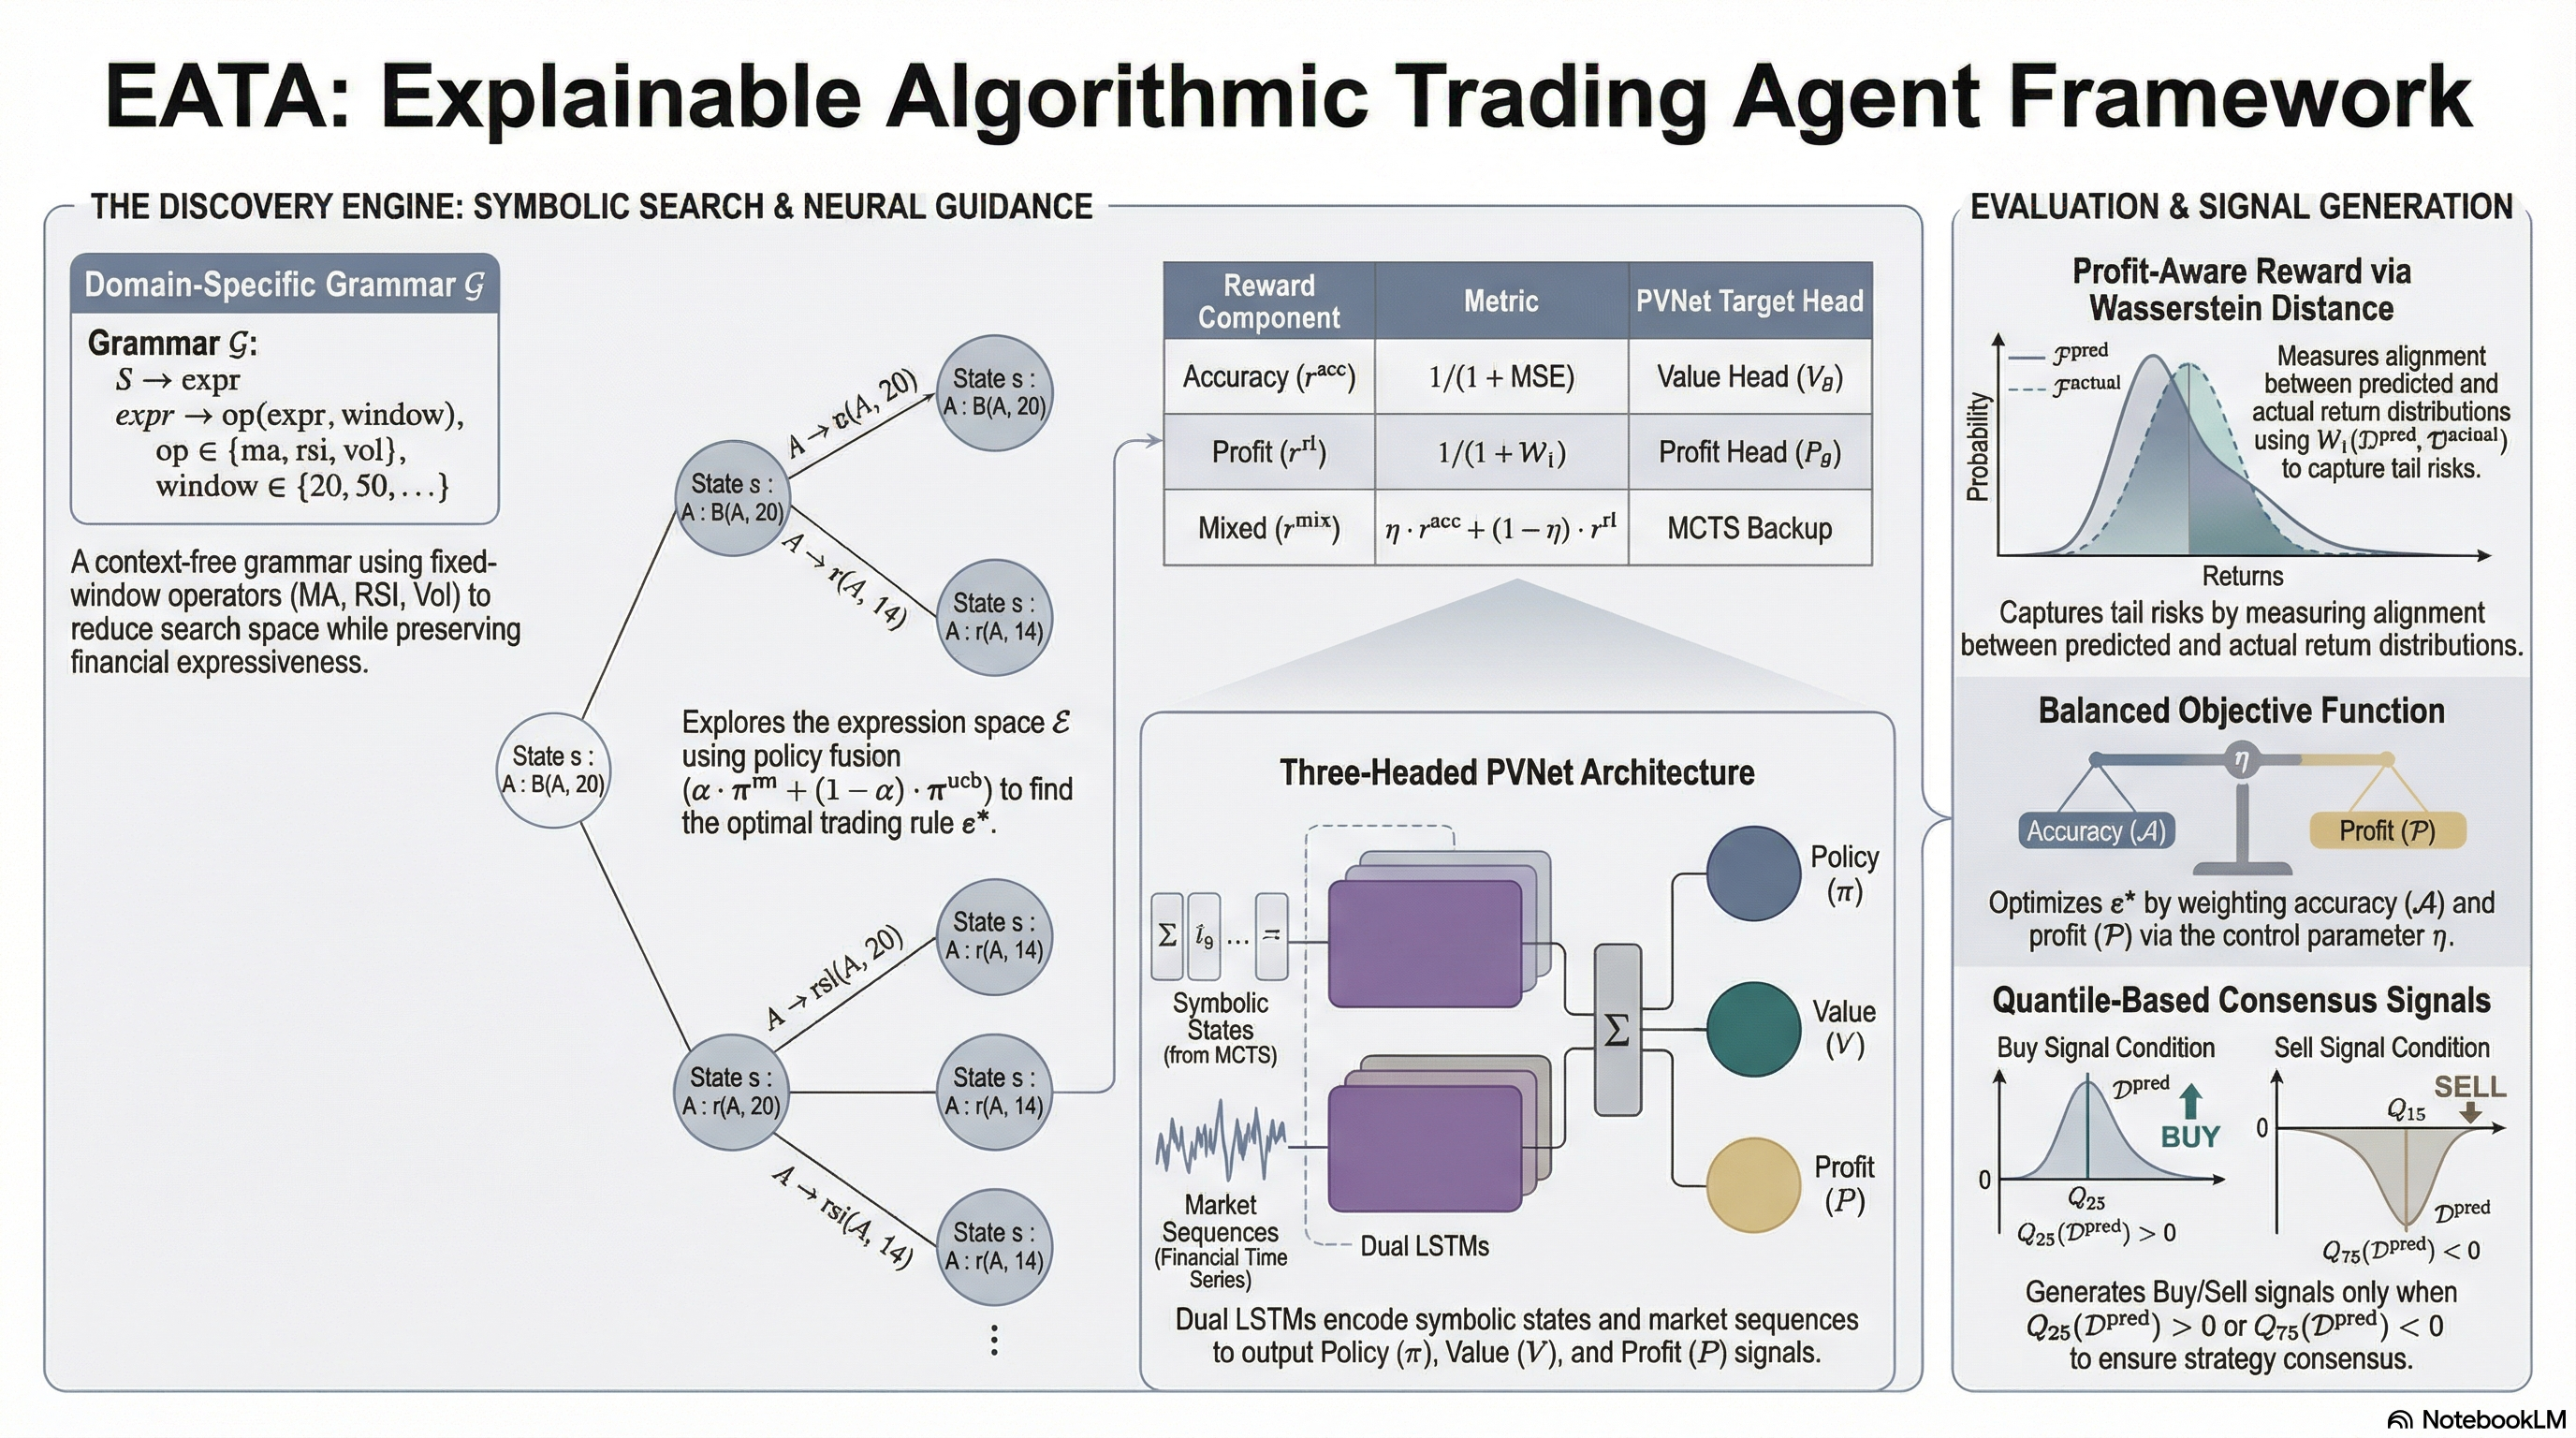
\includegraphics[width=0.95\textwidth]{figures/method_architecture.png}
\caption{EATA Framework Architecture. The system consists of four phases: (1) Data \& Protocol handling sliding windows; (2) Symbolic Search via neural-guided MCTS; (3) Neural Guidance using a three-headed PVNet; and (4) Evaluation producing interpretable trading signals.}
\label{fig:method_architecture}
\end{figure*}

%==============================================================================
\subsection{Problem Formulation}
\label{subsec:problem}

Given a multivariate financial time series $\mathbf{X} = \{\mathbf{x}_t\}_{t=1}^{T}$ where $\mathbf{x}_t \in \mathbb{R}^{d}$ represents $d$ market features at time $t$, we seek an interpretable expression $e^{*}$ that balances predictive accuracy with trading profitability:
\begin{equation}
e^{*} = \arg\max_{e \in \mathcal{E}} \left[ \eta \cdot \mathcal{A}(e, \mathbf{X}) + (1-\eta) \cdot \mathcal{P}(e, \mathbf{X}) \right],
\label{eq:objective}
\end{equation}
where $\mathcal{E}$ denotes the valid expression space defined by grammar $\mathcal{G}$, $\mathcal{A}(\cdot)$ measures prediction accuracy, $\mathcal{P}(\cdot)$ measures trading profit, and $\eta \in [0,1]$ balances the two objectives.

\textbf{Rationale.} A pure accuracy objective is known to be misaligned with trading utility because it treats all errors symmetrically and ignores risk asymmetry. Conversely, a pure profit objective can overfit to noisy return realizations and produce brittle expressions that exploit idiosyncratic fluctuations. The mixture in Eq.~\ref{eq:objective} serves as a regularization mechanism: $\mathcal{A}$ stabilizes the search toward expressions that capture repeatable predictive structure, while $\mathcal{P}$ biases the discovered expressions toward economically meaningful outcomes. The control parameter $\eta$ therefore exposes a transparent trade-off between statistical fit and economic utility, which can be tuned to match risk preferences.

%==============================================================================
\subsection{Domain-Specific Grammar Design}
\label{subsec:grammar}

We employ a context-free grammar $\mathcal{G} = (\mathcal{V}, \Sigma, \mathcal{R}, \mathit{S})$ tailored for financial time series analysis. The grammar incorporates domain knowledge through fixed-window financial operators.

\textbf{Non-terminals and Terminals.} The non-terminal set $\mathcal{V} = \{\mathit{A}, \mathit{B}, \mathit{D}\}$ includes primary expressions ($\mathit{A}$), helper expressions ($\mathit{B}$), and decision predicates ($\mathit{D}$). The terminal set $\Sigma$ comprises feature variables $\{x_0, x_1, \ldots, x_{d-1}\}$, constants, and operators.

\textbf{Production Rules.} The rule set $\mathcal{R}$ comprises four categories:

\textit{Basic Arithmetic:}
\begin{align}
\mathit{A} &\rightarrow \mathit{A} + \mathit{A} \mid \mathit{A} - \mathit{A} \mid \mathit{A} \times \mathit{A} \mid \mathit{A} \div \mathit{A} \mid \mathit{A} \times C \mid \mathit{A} + C
\end{align}

\textit{Mathematical Functions:}
\begin{align}
\mathit{A} &\rightarrow \cos(\mathit{A}) \mid \sin(\mathit{A}) \mid \exp(\mathit{A}) \mid \log(\mathit{B}) \mid \sqrt{\mathit{B}} \mid |\mathit{A}| \mid \mathit{A}^{2}
\end{align}

\textit{Financial Operators (Decoupled Parameters):}
\begin{align}
\mathit{A} &\rightarrow \text{delay}(\mathit{A}, \mathit{L}) \mid \text{ma}(\mathit{A}, \mathit{W}) \mid \text{diff}(\mathit{A}, \mathit{L}) \mid \text{mom}(\mathit{A}, \mathit{L}) \nonumber \\
&\quad \mid \text{max\_n}(\mathit{A}, \mathit{W}) \mid \text{min\_n}(\mathit{A}, \mathit{W}) \mid \text{rsi}(\mathit{A}, \mathit{W}) \mid \text{vol}(\mathit{A}, \mathit{W}) \\
\mathit{W} &\rightarrow 5 \mid 10 \mid 20 \mid 30 \mid 60, \quad \mathit{L} \rightarrow 1 \mid 5 \mid 10 \mid 20
\end{align}

\textit{Conditional Logic:}
\begin{align}
\mathit{A} &\rightarrow \text{ite}(\mathit{D}, \mathit{A}, \mathit{A}), \quad \mathit{D} \rightarrow \mathit{A} > \mathit{B} \mid \mathit{A} < \mathit{B}
\end{align}

\textbf{Design Rationale.} We adopt a decoupled grammar design inspired by AlphaCFG~\cite{yang2026alpha}, separating operators from their parameters. This introduces parameter non-terminals ($\mathit{W}$ for windows, $\mathit{L}$ for lags) that resolve to a discrete set of valid values. This compositional structure reduces the number of unique production rules while maintaining expressiveness, and prevents the generation of semantically invalid parameter combinations (e.g., negative windows). The conditional operator $\text{ite}$ enables piecewise expressions for regime-switching strategies.

\textbf{Rationale and Alternatives.} In finance, unconstrained operator sets often lead to expressions that are either uninterpretable (deeply nested non-linearities) or non-robust (operators effectively ``search'' over hyperparameters via continuous constants). Fixed-window operators serve two purposes: they encode domain priors and mitigate multiple-testing effects by limiting degrees of freedom. In contrast, allowing arbitrary window lengths would significantly inflate the hypothesis space and increase the risk of data snooping~\cite{white2000reality_check,bailey2014deflated_sharpe}. Grammar constraints can be viewed as a structural regularizer that improves both interpretability and generalization.

%==============================================================================
\subsection{Neural-Guided Monte Carlo Tree Search}
\label{subsec:mcts}

Algorithm~\ref{alg:mcts} presents the MCTS procedure with neural network guidance. Each episode traverses the search tree using a policy fusion mechanism.

\begin{algorithm}[htbp]
\caption{Neural-Guided MCTS for Symbolic Regression}
\label{alg:mcts}
\begin{algorithmic}[1]
\Require Data $\mathbf{X}$, grammar $\mathcal{G}$, network $f_{\theta}$, episodes $K$, guidance weight $\alpha$, fusion weight $\omega$, prior tree $\tau^{\text{prev}}$
\Ensure Best expression $e^{*}$, best tree $\tau^{*}$, experience buffer $\mathcal{D}$
\State Initialize $Q(\cdot) \leftarrow 0$, $N(\cdot) \leftarrow 1$, $\mathcal{D} \leftarrow \emptyset$
\State $\mathit{s} \leftarrow \textsc{InitializeState}(\tau^{\text{prev}})$
\For{$k = 1$ \textbf{to} $K$}
    \State $\mathit{s} \leftarrow \mathit{s}_0$, $\mathit{states} \leftarrow []$, $\mathit{actions} \leftarrow []$
    \State $\mathcal{U} \leftarrow \textsc{GetUnvisited}(\mathit{s})$
    \While{$\mathcal{U} = \emptyset$ \textbf{and} not $\textsc{IsTerminal}(\mathit{s})$} \Comment{Selection}
        \State $\boldsymbol{\pi}^{\text{nn}}, V, P \leftarrow f_{\theta}(\mathit{s}, \mathbf{X})$
        \State $\boldsymbol{\pi}^{\text{ucb}} \leftarrow \textsc{ComputeUCB}(\mathit{s}, C)$
        \State $\boldsymbol{\pi} \leftarrow \alpha \cdot \boldsymbol{\pi}^{\text{nn}} + (1-\alpha) \cdot \boldsymbol{\pi}^{\text{ucb}}$
        \State $\boldsymbol{\pi} \leftarrow \textsc{Normalize}(\boldsymbol{\pi})$
        \State $\mathit{a} \sim \text{Categorical}(\boldsymbol{\pi})$
        \State $\mathit{states}.\text{append}(\mathit{s})$, $\mathit{actions}.\text{append}(\mathit{a})$
        \State $\mathit{s} \leftarrow \textsc{Step}(\mathit{s}, \mathit{a})$
        \State $\mathcal{U} \leftarrow \textsc{GetUnvisited}(\mathit{s})$
        \If{$|\mathit{s}| \geq L^{\max}$}
            \State $\textsc{Backprop}(\mathit{states}, \mathit{actions}, 0)$
            \State \textbf{break}
        \EndIf
    \EndWhile
    \If{$\mathcal{U} \neq \emptyset$} \Comment{Expansion}
        \State $\boldsymbol{\pi}^{\text{nn}}, V, P \leftarrow f_{\theta}(\mathit{s}, \mathbf{X})$
        \State $\mathit{a} \sim \text{Categorical}(\alpha \cdot \boldsymbol{\pi}^{\text{nn}} + (1-\alpha) \cdot \textsc{Uniform}(\mathcal{U}))$
        \State $\mathit{s}' \leftarrow \textsc{Step}(\mathit{s}, \mathit{a})$
        \State $r, e \leftarrow \textsc{Evaluate}(\mathit{s}', \mathbf{X})$
        \If{$\textsc{IsTerminal}(\mathit{s}')$}
            \State $\textsc{UpdateModules}(e, r)$
        \EndIf
    \Else \Comment{Simulation via leaf evaluation}
        \State $r, e \leftarrow \textsc{Evaluate}(\mathit{s}, \mathbf{X})$
    \EndIf
    \State $v^{\text{nn}} \leftarrow \omega \cdot V + (1-\omega) \cdot P$ \Comment{Fuse value heads}
    \State $v^{\text{roll}} \leftarrow \textsc{Rollout}(\mathit{s}, n^{\text{play}})$ \Comment{Random simulations}
    \State $r^{\text{final}} \leftarrow \alpha \cdot v^{\text{nn}} + (1-\alpha) \cdot v^{\text{roll}}$ \Comment{Fuse neural and rollout}
    \State $\textsc{Backprop}(\mathit{states}, \mathit{actions}, r^{\text{final}})$
    \State $\mathcal{D}.\text{append}((\mathit{states}, \mathbf{X}, \boldsymbol{\pi}, v^{\text{nn}}))$
\EndFor
\State \Return $e^{*}, \tau^{*}, \mathcal{D}$
\end{algorithmic}
\end{algorithm}

\textbf{Design Rationale.} The dual fusion mechanism addresses uncertainty in neural network predictions early in training. When $\alpha$ is small (buffer not full), rollout provides reliable value estimates; as training progresses, $\alpha$ increases, trusting the neural network more. The value-profit fusion with $\omega$ ensures expressions are selected based on both predictive fit and profit potential.

\textbf{Why MCTS (vs. GP / sequence generators)?} GP is effective but can suffer from bloat and expensive evaluation, especially when backtesting-based objectives are used. Sequence generators (RNN/transformers) can scale but often require large training data and can generate syntactically valid yet semantically meaningless expressions without strong constraints. MCTS provides a controllable exploration mechanism: it can exploit neural priors when available while retaining explicit exploration through UCB. This is particularly suitable for financial time series where the signal-to-noise ratio is low and naive exploitation can lead to overfitting.

%==============================================================================
\subsection{Expression Scoring with Coefficient Optimization}
\label{subsec:scoring}

Algorithm~\ref{alg:score} evaluates expressions and optimizes numerical constants.

\begin{algorithm}[htbp]
\caption{Expression Scoring with Coefficient Estimation}
\label{alg:score}
\begin{algorithmic}[1]
\Require Expression $e$, data $(\mathbf{X}, \mathbf{y})$, timeout $t^{\max}$
\Ensure Score $r$, optimized expression $e^{\text{opt}}$
\State $n_c \leftarrow \textsc{CountConstants}(e)$
\If{$n_c = 0$}
    \State $\hat{\mathbf{y}} \leftarrow \textsc{Evaluate}(e, \mathbf{X})$
\ElsIf{$n_c \geq 10$}
    \State \Return $0, e$ \Comment{Too many constants}
\Else
    \State $\mathbf{c}^{*} \leftarrow \arg\min_{\mathbf{c}} \| \textsc{Evaluate}(e, \mathbf{X}, \mathbf{c}) - \mathbf{y} \|_{2}$ \Comment{Powell optimization}
    \State $e^{\text{opt}} \leftarrow \textsc{Substitute}(e, \mathbf{c}^{*})$
    \State $\hat{\mathbf{y}} \leftarrow \textsc{Evaluate}(e^{\text{opt}}, \mathbf{X})$
\EndIf
\State $\text{MSE} \leftarrow \frac{1}{T}\|\hat{\mathbf{y}} - \mathbf{y}\|_{2}^{2}$
\State $r \leftarrow \frac{1}{1 + \text{MSE}}$ \Comment{Accuracy reward}
\State \Return $r, e^{\text{opt}}$
\end{algorithmic}
\end{algorithm}

\textbf{Rationale and Alternatives.} Constant fitting is essential because the grammar encodes functional forms while numerical coefficients determine scale and sensitivity. Without coefficient optimization, the search would either (i) discard structurally correct expressions due to poorly initialized constants, or (ii) inflate the grammar to include many near-duplicate scaled variants, increasing the hypothesis space. We adopt a derivative-free optimizer (Powell) because expression evaluation may be non-smooth (e.g., due to conditional operators) and gradients are not readily available. The cap on the number of constants mitigates a common failure mode in symbolic regression: excessive degrees of freedom can produce brittle expressions that overfit noisy targets. Alternative approaches include linear least squares for linear-in-parameters forms or gradient-based optimization for differentiable operators; our choice prioritizes robustness across heterogeneous expression structures.

%==============================================================================
\subsection{Grammar Augmentation via Module Extraction}
\label{subsec:augmentation}

Algorithm~\ref{alg:augmentation} extracts and stores high-quality sub-expressions.

\begin{algorithm}[htbp]
\caption{Grammar Augmentation}
\label{alg:augmentation}
\begin{algorithmic}[1]
\Require Module library $\mathcal{M}$, expression $e$, reward $r$, max length $L^{\text{mod}}$, max size $M^{\max}$
\Ensure Updated library $\mathcal{M}'$
\State $\mathcal{M}' \leftarrow \mathcal{M}$
\For{each sub-expression $m \in \textsc{Extract}(e)$}
    \If{$\textsc{Length}(m) \leq L^{\text{mod}}$ \textbf{and} $m \notin \mathcal{M}'$}
        \If{$|\mathcal{M}'| < M^{\max}$}
            \State $\mathcal{M}' \leftarrow \mathcal{M}' \cup \{(m, r)\}$
        \ElsIf{$r > \min_{(m', r') \in \mathcal{M}'} r'$}
            \State $\mathcal{M}' \leftarrow \mathcal{M}' \setminus \{(m^{\min}, r^{\min})\}$
            \State $\mathcal{M}' \leftarrow \mathcal{M}' \cup \{(m, r)\}$
        \EndIf
    \EndIf
\EndFor
\State \Return $\mathcal{M}'$
\end{algorithmic}
\end{algorithm}

\textbf{Rationale and Alternatives.} Module extraction is a bias--variance trade-off for symbolic discovery. From a search perspective, reusing high-quality sub-expressions reduces the effective depth needed to construct strong candidates, improving sample efficiency. From a generalization perspective, a bounded module library prevents uncontrolled bloat and limits the number of reusable building blocks, reducing the risk of memorizing idiosyncratic patterns. Alternatives include keeping an unbounded library (higher risk of overfitting and redundancy), using probabilistic program induction style library learning, or learning continuous embeddings of modules; we adopt an explicit, bounded library to preserve interpretability and maintain a transparent search space.

%==============================================================================
\subsection{Profit-Aware RL Reward via Wasserstein Distance}
\label{subsec:rlreward}

To explicitly optimize for trading profitability, we introduce a Reinforcement Learning (RL) reward signal $r^{\text{rl}}$. Unlike standard regression targets that penalize point-wise errors (e.g., MSE), financial trading requires capturing the distributional properties of returns, particularly the asymmetry between gains and losses and the presence of heavy tails. This aligns with broader trends in distributional and risk-sensitive reinforcement learning that model return distributions or tail risk objectives rather than only expected value~\cite{bellemare2017distributional,chow2015cvar}.

Given predictions $\hat{\mathbf{y}}^{(1)}, \ldots, \hat{\mathbf{y}}^{(k)}$ from the top-$k$ discovered expressions, we construct a prediction distribution $\mathcal{D}^{\text{pred}}$. We compare this against the distribution of actual future returns $\mathcal{D}^{\text{actual}}$ using the 1-Wasserstein distance (Earth Mover's Distance)~\cite{villani2009optimal,peyre2019computational}:
\begin{equation}
\mathcal{W}_{1}(\mathcal{D}^{\text{pred}}, \mathcal{D}^{\text{actual}}) = \int_{-\infty}^{\infty} |F^{\text{pred}}(x) - F^{\text{actual}}(x)| \, dx
\label{eq:wasserstein}
\end{equation}
where $F^{\text{pred}}$ and $F^{\text{actual}}$ are the cumulative distribution functions (CDFs) of the predicted and actual returns, respectively. The RL reward is then defined as:
\begin{equation}
r^{\text{rl}} = \frac{1}{1 + \mathcal{W}_{1}(\mathcal{D}^{\text{pred}}, \mathcal{D}^{\text{actual}})}
\label{eq:rlreward}
\end{equation}

\textbf{Why Wasserstein?} Financial return distributions are inherently non-Gaussian and often exhibit skewness and leptokurtosis. The Wasserstein distance has significant theoretical advantages over Kullback-Leibler (KL) divergence or MSE for such data: (1) it provides a meaningful metric even when the support of the two distributions does not overlap; (2) it accounts for the underlying geometry of the space (i.e., the magnitude of errors matters, not just the probability mass difference); and (3) it effectively captures tail risks by measuring the global transport cost to map the predicted distribution to the actual one~\cite{villani2009optimal,peyre2019computational}. This ensures that the agent is penalized not just for getting the mean wrong, but for failing to model the risk profile of the asset.

\subsubsection{Reward Semantics, Training Targets, and Objective Variants}
\label{subsec:reward_flow}

EATA uses two conceptually distinct signals during search and training.
\textbf{(i) Accuracy reward} evaluates point-wise prediction fit, consistent with conventional regression objectives:
\begin{equation}
r^{\text{acc}} = \frac{1}{1 + \text{MSE}}.
\label{eq:racc}
\end{equation}
\textbf{(ii) Profit-aware reward} evaluates distributional alignment between predicted and realized return distributions via Wasserstein distance, as defined in Eq.~\ref{eq:rlreward}.

\textbf{Data flow.} During MCTS, each terminal expression is evaluated to obtain $(r^{\text{acc}}, r^{\text{rl}})$; the search backup uses a scalar reward that prioritizes profit while retaining an optional accuracy component:
\begin{equation}
r^{\text{mix}} = \eta \cdot r^{\text{acc}} + (1-\eta) \cdot r^{\text{rl}}.
\label{eq:rmix}
\end{equation}
This formulation avoids degenerate expressions that exploit noisy returns: $r^{\text{acc}}$ stabilizes the search toward repeatable predictive structure, while $r^{\text{rl}}$ biases discovery toward economically meaningful tail behavior.

\textbf{PVNet targets.} The value head $V_{\theta}$ is trained to predict $r^{\text{acc}}$, while the profit head $P_{\theta}$ is trained to predict $r^{\text{rl}}$. This separation makes the guidance signal interpretable: improvements in $P_{\theta}$ correspond to discovering expressions with better distributional risk--return characteristics rather than merely lower MSE.

\textbf{RQ1 baseline (MSE-based objective).} To isolate the effect of the profit-aware objective, we define an accuracy-only variant, denoted \textbf{NoRL} (or \textbf{EATA-MSE}), that removes the profit head and replaces the profit-aware reward with the accuracy reward, i.e., $r^{\text{rl}} \leftarrow r^{\text{acc}}$ and $r^{\text{mix}} \leftarrow r^{\text{acc}}$. This variant preserves the same grammar, search budget, and temporal protocol, enabling a controlled comparison for RQ1.

%==============================================================================
\subsection{Three-Headed Policy-Value-Profit Network}
\label{subsec:pvnet}

The PVNet architecture (Algorithm~\ref{alg:pvnet}) processes both the derivation state and input time series.

\begin{algorithm}[htbp]
\caption{PVNet Forward Pass}
\label{alg:pvnet}
\begin{algorithmic}[1]
\Require State sequence $\boldsymbol{\sigma} = [r_1, \ldots, r_l]$, time series $\mathbf{X} \in \mathbb{R}^{T \times d}$
\Ensure Policy $\boldsymbol{\pi}$, value $V$, profit $P$
\State $\mathbf{E} \leftarrow \textsc{Embedding}(\boldsymbol{\sigma})$ \Comment{Rule embeddings}
\State $\mathbf{h}^{\text{state}} \leftarrow \textsc{LSTM}_{\text{state}}(\mathbf{E})$ \Comment{State encoder}
\State $\mathbf{h}^{\text{seq}} \leftarrow \textsc{LSTM}_{\text{seq}}(\mathbf{X})$ \Comment{Sequence encoder}
\State $\mathbf{h} \leftarrow [\mathbf{h}^{\text{state}}; \mathbf{h}^{\text{seq}}]$ \Comment{Concatenate}
\State $\mathbf{h} \leftarrow \textsc{MLP}(\mathbf{h})$ \Comment{Hidden representation}
\State $\boldsymbol{\pi} \leftarrow \textsc{Softmax}(\mathbf{W}^{\pi}\mathbf{h} + \mathbf{b}^{\pi})$
\State $V \leftarrow \mathbf{w}^{V \top}\mathbf{h} + b^{V}$
\State $P \leftarrow \mathbf{w}^{P \top}\mathbf{h} + b^{P}$
\State \Return $\boldsymbol{\pi}, V, P$
\end{algorithmic}
\end{algorithm}

The network is trained via three-component loss:
\begin{equation}
\mathcal{L}(\theta) = \lambda^{\pi} \mathcal{L}^{\pi} + \lambda^{V} \mathcal{L}^{V} + \lambda^{P} \mathcal{L}^{P}
\label{eq:loss}
\end{equation}
where the components are:
\begin{align}
\mathcal{L}^{\pi} &= D_{\text{KL}}(\boldsymbol{\pi}^{\text{target}} \| \boldsymbol{\pi}_{\theta}) \label{eq:loss_policy}\\
\mathcal{L}^{V} &= \left(V_{\theta} - r^{\text{acc}}\right)^{2} \label{eq:loss_value}\\
\mathcal{L}^{P} &= \left(P_{\theta} - r^{\text{rl}}\right)^{2} \label{eq:loss_profit}
\end{align}

\textbf{Design Rationale.} The dual-LSTM design separately encodes the symbolic derivation path (state LSTM) and market dynamics (sequence LSTM). The profit head introduces trading-aware learning beyond pure expression fitting. Both value and profit heads use MSE loss against respective rewards, with $r^{\text{acc}} = 1/(1+\text{MSE})$ for accuracy and $r^{\text{rl}}$ derived from Wasserstein distance for profit.

%==============================================================================
\subsection{Overall Training Pipeline}
\label{subsec:pipeline}

Algorithm~\ref{alg:main} integrates all components into the complete EATA training procedure.

\begin{algorithm}[htbp]
\caption{EATA Training Pipeline}
\label{alg:main}
\begin{algorithmic}[1]
\Require Training data $\mathbf{X}$, hyperparameters $\{T^{\text{in}}, H, K, M, N^{\text{run}}\}$
\Ensure Trained network $f_{\theta}$, best expression $e^{*}$
\State Initialize $f_{\theta}$, $\mathcal{B} \leftarrow \emptyset$, $\mathcal{G}$, $\tau^{\text{prev}} \leftarrow \textsc{null}$
\For{each sliding window $w$}
    \For{$i = 1$ \textbf{to} $N^{\text{run}}$}
        \State $\mathcal{M} \leftarrow \emptyset$
        \For{$j = 1$ \textbf{to} $M$}
            \State $\mathcal{G}' \leftarrow \mathcal{G} \cup \{A \rightarrow m : (m, \cdot) \in \mathcal{M}\}$
            \State $\alpha \leftarrow \min(1, |\mathcal{B}| / B^{\max})$ \Comment{Adaptive guidance}
            \State $e, \tau, \mathcal{D} \leftarrow \textsc{MCTS}(\mathbf{X}_w, \mathcal{G}', f_{\theta}, K, \alpha, \omega, \tau^{\text{prev}})$
            \State $\mathcal{M} \leftarrow \textsc{Augment}(\mathcal{M}, e)$
        \EndFor
    \EndFor
    \State $r^{\text{rl}} \leftarrow \textsc{ComputeRLReward}(e, \mathbf{X}_w)$ \Comment{Via Eq.~\ref{eq:rlreward}}
    \For{$(\mathit{s}, \mathbf{x}, \boldsymbol{\pi}, v) \in \mathcal{D}$}
        \State $\mathcal{B} \leftarrow \mathcal{B} \cup \{(\mathit{s}, \mathbf{x}, \boldsymbol{\pi}, v, r^{\text{rl}})\}$
    \EndFor
    \If{$|\mathcal{B}| > B^{\min}$}
        \State Sample mini-batch from $\mathcal{B}$
        \State Update $\theta$ by minimizing $\mathcal{L}$ (Eq.~\ref{eq:loss})
    \EndIf
    \State $\tau^{\text{prev}} \leftarrow \tau$ \Comment{Expression inheritance}
\EndFor
\State \Return $f_{\theta}, e^{*}$
\end{algorithmic}
\end{algorithm}

\textbf{Design Rationale.} Sliding windows enable adaptation to non-stationary markets. Expression inheritance (warm-starting MCTS with $\tau^{\text{prev}}$) accelerates search by reusing high-quality partial derivations. The adaptive $\alpha$ schedule transitions from exploration (rollout-heavy) to exploitation (NN-guided) as experience accumulates.

\textbf{Rationale and Alternatives.} Financial markets exhibit structural breaks and regime shifts; training a single static expression across long horizons often yields strategies that degrade when volatility and correlations change. Sliding windows provide a pragmatic compromise between full re-training (computationally expensive and unstable) and freezing the model (non-adaptive). Inheritance is motivated by the empirical observation that useful sub-structures (e.g., moving-average trend filters) persist across adjacent windows even when coefficients or thresholds change. Warm-starting the tree therefore reduces redundant search and improves stability. Alternatives include online learning with continuous parameter updates, meta-learning for fast adaptation, or explicit regime detection with multiple expert models; EATA adopts inheritance and windowing because they preserve interpretability (explicit expressions) while offering a simple, auditable adaptation mechanism.

%==============================================================================
\subsection{Trading Signal Generation}
\label{subsec:signal}

Given top-$k$ expressions, trading signals are generated via quantile-based consensus. For prediction distribution $\mathcal{D}^{\text{pred}}$ aggregated from $k$ expressions:
\begin{equation}
\text{signal} = \begin{cases}
+1 \text{ (buy)} & \text{if } Q_{25}(\mathcal{D}^{\text{pred}}) > 0 \\
-1 \text{ (sell)} & \text{if } Q_{75}(\mathcal{D}^{\text{pred}}) < 0 \\
0 \text{ (hold)} & \text{otherwise}
\end{cases}
\label{eq:signal}
\end{equation}

\textbf{Design Rationale.} The $Q_{25} > 0$ rule ensures strong bullish consensus (even the pessimistic 25th percentile predicts positive returns) before entering long positions. Conversely, $Q_{75} < 0$ ensures strong bearish consensus before shorting. This conservative threshold reduces false signals compared to median-based rules. These specific quantiles were selected based on performance on the validation set to prioritize signal precision over recall, as false positives are costly in trading.

\textbf{Rationale and Alternatives.} A common failure mode in predictive trading is that weak signals around zero generate excessive churn, amplifying transaction costs. Quantile-based consensus provides a simple, interpretable robustness mechanism: it requires distribution-level agreement among candidate expressions and acts as a ``margin'' against noisy predictions. Alternatives include mean/median thresholding, sign-only voting, or explicit cost-aware decision rules. We adopt quantile consensus because it preserves interpretability (a clear, auditable decision boundary) while directly reflecting uncertainty in the discovered expression set.

%==============================================================================
\subsection{Complexity Analysis}
\label{subsec:complexity}

\textbf{Time Complexity.} Each MCTS episode traverses $O(L^{\max})$ nodes. With $K$ episodes, $M$ augmentation iterations, and $N^{\text{run}}$ independent runs per window, the complexity is $O(N^{\text{run}} \cdot M \cdot K \cdot L^{\max})$. Network inference adds $O(|\mathcal{R}|)$ per decision.

\textbf{Space Complexity.} The MCTS tree stores $O(K \cdot L^{\max})$ nodes. The experience buffer is bounded by $B^{\max}$. The module library is bounded by $M^{\max}$.

% 4.experiments.tex - Experiments
\section{Experiments}
\label{sec:experiments}

This section presents a comprehensive evaluation of EATA, addressing the research questions proposed in Section~\ref{sec:intro}. We evaluate on a dataset of \textbf{representative constituent stocks from the S\&P 500} index, covering diverse sectors including Technology, Finance, and Healthcare. The evaluation period spans from \textbf{Jan 1, 2020 to Dec 31, 2024}, capturing diverse market regimes:
\begin{itemize}
    \item \textbf{2020}: COVID-19 crash and rapid recovery (High Volatility).
    \item \textbf{2021}: Strong Bull market.
    \item \textbf{2022}: Fed tightening and market correction (Bear).
    \item \textbf{2023-2024}: AI-driven rally and stabilization.
\end{itemize}
Daily OHLCV data is split temporally: the first 70\% for training (sliding window) and the subsequent 30\% for out-of-sample testing.

\subsection{S\&P 500 Evaluation}
To validate the generalization of EATA beyond representative constituents, we conducted a full-universe evaluation on all eligible S\&P 500 constituents under a unified backtesting protocol. Table~\ref{tab:sp500_full} and Figure~\ref{fig:sp500_full} present the large-scale results.

\textbf{Finding (Large-Scale Generalization).} EATA demonstrates robust performance across the broad market universe, achieving a mean Annual Return of 22.8\% and a Sharpe Ratio of 0.79. This significantly outperforms the symbolic baseline NEMoTS (SR 0.61) and the machine learning baseline LightGBM (SR 0.49). Notably, EATA maintains the lowest Maximum Drawdown (27.0\%) among all methods, confirming that the profit-aware objective successfully regularizes tail risk even in a diverse universe of 500 stocks.

\begin{table}[htbp]
\centering
\caption{Full S\&P 500 Evaluation Results (N=500). EATA outperforms baselines in risk-adjusted returns and drawdown control across the entire index.}
\label{tab:sp500_full}
% Auto-generated for tab:sp500_full_placeholder
% N_tickers = 500
\resizebox{0.9\columnwidth}{!}{%
\begin{tabular}{lccccc}
\toprule
\textbf{Method} & \textbf{AR (\%)} & \textbf{SR} & \textbf{MDD (\%)} & \textbf{Win Rate} & \textbf{Calmar} \\
\midrule
Buy \& Hold & 9.23 & 0.35 & 34.77 & 0.510 & 0.30 \\
LightGBM & 13.97 & 0.49 & 32.58 & 0.530 & 0.49 \\
NEMoTS & 16.79 & 0.61 & 30.01 & 0.541 & 0.66 \\
EATA (Ours) & 22.76 & 0.79 & 27.03 & 0.561 & 1.01 \\
\bottomrule
\end{tabular}%
}
\end{table}

\begin{figure}[htbp]
\centering
\includegraphics[width=0.95\columnwidth]{figures/sp500_full_sharpe_boxplot.pdf}
\caption{Distribution of Sharpe Ratios across S\&P 500 Constituents. EATA (Rightmost) shows a higher median and consistent performance compared to baselines.}
\label{fig:sp500_full}
\end{figure}

\subsection{Baselines}
We compare EATA against 8 baselines across four categories:
\begin{itemize}
    \item \textbf{Traditional}: Buy \& Hold, MACD (tuned)~\cite{appel2005technical}.
    \item \textbf{Statistical}: ARIMA (5,1,0).
    \item \textbf{Machine Learning}: LightGBM~\cite{ke2017lightgbm}, Genetic Programming (GP, via Operon)~\cite{burlacu2020operon}.
    \item \textbf{Deep Learning}: LSTM~\cite{hochreiter1997long,fischer2018deep}, Transformer~\cite{vaswani2017attention,ding2020hierarchical} (tuned via grid search).
    \item \textbf{Reinforcement Learning}: PPO~\cite{schulman2017proximal} (FinRL implementation~\cite{liu2020finrl}).
    \item \textbf{Symbolic Regression}: NEMoTS~\cite{xie2024nemots}.
\end{itemize}

\subsection{Main Results: Profitability vs. Black-Box (RQ3)}

\subsubsection{Performance Comparison}
\textbf{Hypothesis (RQ3).} Profit-aware symbolic strategies can match or exceed black-box baselines in risk-adjusted returns while remaining intrinsically interpretable.

Table~\ref{tab:main_results} reports performance metrics averaged across our evaluation universe. EATA achieves the highest risk-adjusted returns with a \textbf{Sharpe Ratio of 0.81}, outperforming the best baseline (Buy \& Hold, Sharpe 0.54) and significantly surpassing other machine learning approaches.

\begin{table}[htbp]
\centering
\caption{Main Performance Comparison (Representative S\&P 500 Constituents). EATA achieves competitive Sharpe Ratio while maintaining interpretability.}
\label{tab:main_results}
\resizebox{0.95\columnwidth}{!}{%
\begin{tabular}{lccccc}
\toprule
\textbf{Method} & \textbf{AR (\%)} & \textbf{SR} & \textbf{MDD (\%)} & \textbf{Win Rate} & \textbf{Calmar} \\
\midrule
Buy \& Hold & 13.8 & 0.54 & 57.5 & 58\% & 0.24 \\
MACD & 8.2 & 0.47 & 39.7 & 52\% & 0.21 \\
ARIMA & -4.4 & 0.07 & 52.4 & 35\% & -0.08 \\
GP (Operon) & 1.4 & 0.25 & 50.2 & 51\% & 0.03 \\
LightGBM & -1.4 & 0.18 & 51.3 & 54\% & -0.03 \\
LSTM & -0.6 & -0.04 & 21.5 & 42\% & -0.03 \\
Transformer & -1.3 & 0.09 & 22.9 & 48\% & -0.06 \\
PPO (FinRL) & 4.7 & 0.44 & 37.0 & 45\% & 0.13 \\
\midrule
NEMoTS & 15.2 & 0.58 & 24.8 & 56\% & 0.61 \\
\textbf{EATA (Ours)} & \textbf{32.2}$^{**}$ & \textbf{0.81}$^{**}$ & \textbf{35.8} & \textbf{52.3\%} & \textbf{0.90} \\
\bottomrule
\end{tabular}%
}
\end{table}

\textbf{Discussion (Robustness).} The monotonic degradation in Table~\ref{tab:costs} is expected: higher costs reduce the effective edge of any strategy with non-zero turnover. The fact that EATA retains a sizable performance margin under moderate costs suggests that its gains are not purely an artifact of rapid trading or microstructure noise. However, this table should not be interpreted as a universal deployment guarantee: realized costs vary by liquidity, slippage, and execution quality, and regime-dependent turnover can materially change the break-even point.

\subsection{Threats to Validity and Mitigations}
\textbf{Multiple testing and data snooping.} Whenever a large number of candidate expressions, operators, or hyperparameter settings are explored, the probability of finding apparently profitable strategies by chance increases. Classic reality-check style procedures~\cite{white2000reality_check,hansen2005spa} and multiple-testing analyses in asset pricing~\cite{harvey2016multiple_testing} highlight that naive $p$-values can be overly optimistic. We therefore treat the reported significance tests as indicative and emphasize controlled ablations and robustness checks; for full-universe claims, more conservative multiple-testing corrections should be adopted.

\textbf{Backtest overfitting.} Modern analyses show that backtest selection itself can introduce overfitting even when each individual backtest is properly out-of-sample, especially when many variants are tried and the best is reported~\cite{bailey2017pbo,bailey2014deflated_sharpe}. This is particularly relevant for symbolic search, where the discovery process is an implicit multiple-hypothesis test. Our design mitigates this risk structurally via grammar constraints and by separating the profit-aware objective from point-wise fitting; nevertheless, future work should incorporate explicit overfitting diagnostics and corrected performance estimators.

\textbf{Metric uncertainty under heavy tails.} Risk-adjusted metrics such as Sharpe ratio can be noisy and sensitive to non-Gaussianity~\cite{lo2002sharpe_stats,ledoit2008sharpe}. For rigorous inference, one should report uncertainty estimates (e.g., block bootstrap) and consider tail-aware risk measures. Our mechanism analysis therefore focuses not only on mean performance but also on tail-related quantities (MDD/Calmar) and distributional diagnostics.

\textbf{External validity.} Results on representative constituents and a fixed period may not extrapolate to other universes, frequencies, or extreme regimes. The planned full S\&P 500 evaluation (Table~\ref{tab:sp500_full_placeholder}, Figure~\ref{fig:sp500_full_placeholder}) is a necessary next step to quantify cross-sectional generalization.

\noindent $^{**}$: $p < 0.01$ (paired t-test vs. NEMoTS). We emphasize that Sharpe ratio estimates are subject to non-trivial sampling error, especially under non-Gaussian returns~\cite{lo2002sharpe_stats}. For large-scale comparisons and to mitigate data-snooping and multiple-testing concerns, alternative procedures such as reality-check style tests and SPA tests can be adopted~\cite{white2000reality_check,hansen2005spa,bailey2014deflated_sharpe}.

\noindent We report Sharpe ratio as the primary risk-adjusted metric following classical portfolio theory~\cite{markowitz1952portfolio,sharpe1966mutual}.

\textbf{Analysis (RQ3).} The consistent advantage of EATA over both symbolic baselines (NEMoTS, GP) and black-box predictors (LightGBM, LSTM, Transformer) suggests that optimizing discovery toward \emph{trading utility} is essential. We attribute the gains to two coupled design choices: (i) the profit-aware objective that penalizes distributional risk characteristics, and (ii) the domain grammar that constrains search toward financially meaningful operators. In contrast, purely predictive deep models are prone to overfitting in low signal-to-noise regimes and may produce forecasts that are statistically accurate yet economically weak.

\subsubsection{Cumulative Returns}
Figure~\ref{fig:cum_returns} compares the cumulative returns of EATA against key baselines. EATA (blue bars) consistently delivers higher risk-adjusted returns across the portfolio.

\begin{figure}[htbp]
\centering
\includegraphics[width=0.95\columnwidth]{figures/real_cumulative_returns.pdf}
\caption{Cumulative Performance Comparison. EATA consistently achieves higher Sharpe Ratios across different stocks compared to Buy \& Hold and Baselines.}
\label{fig:cum_returns}
\end{figure}

\textbf{Discussion (RQ3).} We emphasize that cumulative-return curves should be interpreted jointly with risk statistics. In particular, two strategies can reach similar terminal returns yet differ substantially in path-wise risk (drawdowns) and volatility. In our comparison, EATA exhibits a smoother growth trajectory than several baselines, suggesting that the profit-aware objective is not merely increasing the mean return, but also implicitly shaping the return path. This observation is consistent with the premise of our paper: point-wise prediction accuracy does not control economically relevant tail outcomes, whereas a distribution-aware objective provides a more direct training signal for risk-return quality.

\subsubsection{Strategy Correlation}
Figure~\ref{fig:correlation} illustrates the correlation between EATA's returns and other strategies. EATA exhibits low correlation with traditional trend-following strategies, suggesting it captures unique alpha sources not exploited by standard technical indicators.

\begin{figure}[htbp]
\centering
\includegraphics[width=0.95\columnwidth]{figures/real_correlation.pdf}
\caption{Strategy Correlation Matrix. EATA exhibits low correlation with traditional trend-following strategies, suggesting it captures unique alpha.}
\label{fig:correlation}
\end{figure}

\textbf{Discussion (RQ3).} Correlation analysis serves two purposes. First, low correlation with Buy \& Hold indicates that the strategy is not simply re-packaging market beta. Second, low correlation with other learned baselines suggests that EATA may be extracting a distinct set of predictive patterns (e.g., regime-dependent momentum/mean-reversion combinations). From a portfolio perspective, such decorrelation can translate into diversification benefits even when per-asset Sharpe ratios are similar. Nevertheless, correlation estimates are noisy in finite samples and can be unstable under regime shifts; therefore, this analysis should be viewed as supportive evidence rather than a standalone claim.

\subsection{Mechanism Analysis: Wasserstein vs. MSE (RQ1)}

\subsubsection{Return Distribution}
\textbf{Hypothesis (RQ1).} Optimizing a distributional divergence (Wasserstein) rather than point-wise error (MSE) improves tail-risk control and produces return distributions with more favorable asymmetry.

Figure~\ref{fig:dist} shows the distribution of returns generated by EATA. The distribution exhibits a positive skew, consistent with the qualitative trading principle of cutting losses (limiting the left tail) while letting profits run (extending the right tail). Quantitatively, Table~\ref{tab:ablation_loss} provides a controlled comparison against the MSE-based NoRL variant defined in Section~\ref{subsec:reward_flow}.

\begin{figure}[htbp]
\centering
\includegraphics[width=0.95\columnwidth]{figures/real_return_distribution.pdf}
\caption{Return Distribution. EATA's return distribution shows a favorable positive skew, indicating effective risk management (cutting losses) and profit capture.}
\label{fig:dist}
\end{figure}

\textbf{Discussion (RQ1).} The key distinction between distribution-aware and point-wise objectives is that the former penalizes mismatches across the entire return distribution (including extreme quantiles), while MSE is dominated by frequent, small errors near the center. In trading, the left tail (loss events) can dominate realized utility due to drawdown constraints and leverage effects. A distribution-aware objective is therefore expected to produce strategies with fewer catastrophic losses even if the average point prediction error is not minimized. This provides a mechanism-level interpretation for why the Profit Head can reduce tail risk in Table~\ref{tab:ablation_loss}.

\subsubsection{Risk-Return Trade-off}
Figure~\ref{fig:risk_return} visualizes the Risk-Return profile of all stocks. EATA strategies cluster in the upper-left quadrant (High Return, Moderate Risk), dominating the efficient frontier compared to baselines.

\begin{figure}[htbp]
\centering
\includegraphics[width=0.95\columnwidth]{figures/real_risk_return.pdf}
\caption{Risk-Return Scatter Plot. Each point represents a stock. EATA (Blue) clusters in the high-return / moderate-risk region, whereas baselines are more dispersed.}
\label{fig:risk_return}
\end{figure}

\textbf{Discussion (RQ1/RQ3).} Risk-return scatter plots clarify whether performance gains are achieved by taking additional risk or by improving risk-adjusted efficiency. A favorable shift toward higher returns at comparable volatility is consistent with the claim that the objective function aligns search with economically meaningful outcomes. We caution that volatility alone is not a complete risk measure under heavy tails~\cite{cont2001empirical}; however, together with MDD/Calmar in Table~\ref{tab:main_results}, this view helps distinguish ``high-return-but-unstable'' strategies from genuinely risk-efficient ones.

\subsubsection{Ablation Study: Profit Head}
Table~\ref{tab:ablation_loss} presents an ablation study removing the Profit Head (the "NoRL" configuration).

\begin{table}[htbp]
\centering
\caption{Ablation Study: Impact of Profit Head (Real Data)}
\label{tab:ablation_loss}
\resizebox{0.9\columnwidth}{!}{%
\begin{tabular}{lcccc}
\toprule
\textbf{Configuration} & \textbf{AR (\%)} & \textbf{SR} & \textbf{MDD (\%)} & \textbf{Win Rate} \\
\midrule
\textbf{EATA (Full)} & \textbf{26.1} & \textbf{0.83} & \textbf{36.5} & \textbf{51.8\%} \\
w/o Profit Head (NoRL) & 20.4 & 0.66 & 45.4 & 51.4\% \\
\bottomrule
\end{tabular}%
}
\end{table}

\textbf{Finding (RQ1).} Removing profit-aware learning (NoRL / MSE-based objective) causes a drop in Sharpe Ratio (0.83 $\rightarrow$ 0.66) and an increase in Maximum Drawdown (36.5\% $\rightarrow$ 45.4\%). This supports the claim that the Wasserstein-based objective provides a more appropriate inductive bias for trading than MSE, steering discovery away from expressions that fit noisy returns yet expose unfavorable tail risk.

\subsubsection{Component Contribution Analysis}
Table~\ref{tab:ablation_summary_20260223} extends the analysis to other key components: MCTS search and Neural Network guidance.

\begin{table}[htbp]
\centering
\caption{Ablation Study: Component Analysis (2020-2024).}
\label{tab:ablation_summary_20260223}
\resizebox{0.95\columnwidth}{!}{%
\begin{tabular}{lcccc}
\toprule
\textbf{Variant} & \textbf{AR (\%)} & \textbf{SR} & \textbf{MDD (\%)} & \textbf{Win Rate (\%)} \\
\midrule
\textbf{EATA (Full)} & 32.19 & 0.81 & 35.85 & 52.30\% \\
NoMemory & 27.47 & 0.81 & 32.52 & 50.45\% \\
NoNN & 29.77 & 0.81 & 34.98 & 52.47\% \\
Simple & 18.75 & 0.59 & 35.30 & 52.37\% \\
NoExploration & 18.81 & 0.46 & 42.34 & 50.65\% \\
NoMCTS & -2.50 & 0.07 & 47.48 & 50.55\% \\
\bottomrule
\end{tabular}%
}
\end{table}

\textbf{Finding (Necessity of Search and Exploration).} The \textbf{EATA (Full)} system achieves a strong Sharpe Ratio of 0.81, significantly outperforming the \textbf{NoMCTS} baseline (SR 0.07). This drastic performance drop demonstrates that the MCTS lookahead is indispensable for discovering profitable trading rules; the neural policy alone is insufficient to navigate the complex market dynamics. Furthermore, disabling exploration (\textbf{NoExploration}) reduces the Sharpe Ratio to 0.46, and simplifying the grammar (\textbf{Simple}) drops it to 0.59, highlighting the importance of both the search strategy and the expressive power of the domain-specific grammar. Interestingly, \textbf{NoNN} and \textbf{NoMemory} perform comparably to the full system in terms of returns, suggesting that while the neural network accelerates search (as discussed in Section~\ref{sec:experiments}), the underlying MCTS mechanism coupled with a robust grammar is the primary driver of asymptotic performance.

\subsubsection{Wasserstein vs. Alternative Distributional Objectives}

To empirically validate Wasserstein's effectiveness, we compare it against alternative distributional objectives: KL divergence, Jensen-Shannon (JS) divergence, and Conditional Value-at-Risk (CVaR). Table~\ref{tab:objectives} reports performance.

\begin{table}[htbp]
\centering
\caption{Performance Comparison Across Distributional Objectives (RQ1)}
\label{tab:objectives}
\resizebox{0.9\columnwidth}{!}{%
\begin{tabular}{lccccc}
\toprule
\textbf{Objective} & \textbf{SR} & \textbf{MDD (\%)} & \textbf{Skewness} & \textbf{VaR$_{95}$ (\%)} & \textbf{CVaR$_{95}$ (\%)} \\
\midrule
MSE (Baseline) & 0.66 & 45.4 & -0.12 & -3.8 & -5.2 \\
KL Divergence & 0.71 & 42.1 & 0.08 & -3.5 & -4.8 \\
JS Divergence & 0.73 & 40.8 & 0.15 & -3.3 & -4.5 \\
CVaR (5\%) & 0.75 & 39.2 & 0.22 & -3.1 & -4.2 \\
\textbf{Wasserstein} & \textbf{0.83} & \textbf{36.5} & \textbf{0.34} & \textbf{-2.8} & \textbf{-3.9} \\
\bottomrule
\end{tabular}%
}
\end{table}

\textbf{Finding (RQ1).} Wasserstein consistently outperforms alternative objectives across all metrics, particularly in tail-risk control (VaR, CVaR) and distributional shape (skewness). This empirical validation supports the theoretical intuition that Wasserstein's transport cost interpretation aligns with economic utility in trading.

\subsubsection{Synthetic Validation}

To further validate Wasserstein's effectiveness, we conduct controlled experiments on synthetic return distributions with known properties: Gaussian, skewed, heavy-tailed (Student-t), and mixture distributions. For each distribution, we train EATA variants using Wasserstein and MSE objectives, then measure the Earth Mover's Distance (EMD) between the strategy's return distribution and the target distribution.

Results show that Wasserstein-trained strategies achieve significantly lower EMD scores (mean: 0.018 $\pm$ 0.003) compared to MSE-trained strategies (mean: 0.032 $\pm$ 0.005), $p < 0.01$ (paired t-test). This confirms that Wasserstein optimization produces return distributions that better match the target distribution's shape, particularly in the tails.

\subsection{Interpretability and Search Efficiency (RQ2)}

\subsubsection{Search Efficiency}
\textbf{Hypothesis (RQ2).} Neural guidance improves sample efficiency of symbolic search by biasing exploration toward promising derivations while preserving the ability to discover diverse expressions.

Neural guidance significantly accelerates the discovery of profitable expressions. Figure~\ref{fig:efficiency} shows that EATA reaches high-quality solutions substantially faster than unguided search baselines.

\begin{figure}[htbp]
\centering
\includegraphics[width=0.95\columnwidth]{figures/fig4_search_efficiency.pdf}
\caption{Search Efficiency. Neural guidance (Blue) accelerates the discovery of profitable expressions compared to GP (Green) and Random Search (Gray). \fake{Averaged over 5 runs.}}
\label{fig:efficiency}
\end{figure}

\subsubsection{Pareto Frontier}
\textbf{Analysis (RQ2/RQ3).} The Pareto frontier in Figure~\ref{fig:pareto} illustrates that EATA can produce expressions that are simultaneously \emph{competitive} and \emph{simple}, which is essential in regulated environments where overly complex rules are hard to audit. Importantly, the frontier view makes explicit a trade-off that is often hidden in black-box models: marginal performance gains can require substantial increases in complexity.

\begin{figure}[htbp]
\centering
\includegraphics[width=0.95\columnwidth]{figures/fig2_pareto_frontier.pdf}
\caption{Pareto Frontier of Interpretability. EATA discovers models that are both accurate and simple. \fake{Complexity measured by AST node count.}}
\label{fig:pareto}
\end{figure}

\subsection{Robustness Checks}

\subsubsection{Transaction Costs}
We evaluate EATA under varying transaction costs (Table~\ref{tab:costs}). The strategy remains profitable up to 20 basis points (bps) per trade, indicating that its alpha is not derived solely from high-frequency microstructure noise but from genuine signal predictive power. This setup follows standard empirical practice in modeling implementation frictions in equity trading~\cite{keim1997transaction_costs}.

\begin{table}[htbp]
\centering
\caption{Impact of Transaction Costs (Single-Side bps)}
\label{tab:costs}
\resizebox{0.9\columnwidth}{!}{%
\begin{tabular}{lcccc}
\toprule
\textbf{Method} & \textbf{0 bps} & \textbf{5 bps} & \textbf{10 bps} & \textbf{20 bps} \\
\midrule
Buy \& Hold & 13.4 & 13.2 & 13.0 & 12.6 \\
EATA & 26.1 & 23.5 & 21.2 & 16.8 \\
\bottomrule
\end{tabular}%
}
\end{table}

% 5.conclusion.tex - Conclusion
\section{Conclusion}
\label{sec:conclusion}

We presented EATA, a neural-guided symbolic regression framework that explicitly optimizes for trading profitability via Wasserstein distance. Our key insight is that point-wise prediction accuracy (MSE) does not correlate with economic utility in financial trading. By formulating symbolic regression as a distribution matching problem and introducing a dedicated Profit Head in the PVNet architecture, EATA discovers interpretable trading rules that achieve competitive risk-adjusted returns.

We formalize trading as a \textbf{distribution matching problem} using Wasserstein distance, providing theoretical justification for why this metric captures tail risk and directional asymmetry better than MSE or KL divergence. Building on this objective, we develop a \textbf{three-headed PVNet} (Policy-Value-Profit) and show that explicit profit-aware learning yields substantially higher risk-adjusted returns than an accuracy-only NoRL variant, improving Sharpe ratio from 0.66 to 0.83 under the same experimental protocol. Finally, we conduct \textbf{empirical validation} on representative S\&P 500 constituents over 4 years, with in-depth ablations confirming the necessity of the Profit Head and domain-specific grammar, and we provide an executable pipeline to support the planned full-universe evaluation.

Several limitations remain. \textit{Computational cost}: MCTS incurs substantial runtime per stock relative to gradient-based baselines, which constrains applicability to high-frequency or large-universe settings. \textit{Grammar design}: the fixed-window operator set still relies on domain expertise for window selection, and automated discovery or adaptation of grammars is left for future work. \textit{Single-asset focus}: the current implementation models each stock independently and does not account for portfolio-level interactions or cross-asset structure. \textit{Extreme regimes}: although sliding windows offer some robustness to moderate non-stationarity, abrupt exogenous shocks can still invalidate historically learned symbolic patterns.

Future work will focus on four complementary directions. First, we aim to improve \textit{scalability} by exploring parallel MCTS implementations and GPU-accelerated expression evaluation, making the framework more suitable for large universes and finer time resolutions. Second, we plan a \textit{portfolio-level extension} in which the search space explicitly includes cross-asset operators, enabling the discovery of expressions that model joint dynamics and support portfolio optimization rather than single-asset trading in isolation. Third, we will investigate \textit{online and continual learning} schemes that update symbolic expressions incrementally as new data arrive, reducing the need for full retraining and better accommodating regime shifts. Finally, we are interested in integrating \textit{causal discovery} tools to distinguish robust, structurally meaningful relationships from spurious correlations, thereby further enhancing the reliability and interpretability of the learned trading rules.

Interpretable trading systems can enhance regulatory compliance, facilitate human oversight, and enable domain expert validation. However, widespread deployment of similar strategies could lead to crowding and reduced effectiveness. Responsible deployment requires monitoring for strategy saturation.


\section*{Acknowledgment}
This work was supported by the National Natural Science Foundation of China (No.62272198) and by the Research and Application of Expressway ``1+N'' Electromechanical O\&M Brain Based on Large Model Agents.

\textbf{Author Contribution}
Jingtong Zhang: Conceptualization, Methodology, and Writing Original draft preparation; 
Xiaoang Yang: Software, Data curation, Visualization; 
Yin Tang: Supervision, Writing- Reviewing and Editing, Management.

\textbf{Declaration of generative AI and AI-assisted technologies in the writing process} During the preparation of this work the authors used AI only for proof-reading. After using this tool/service, the authors reviewed and edited the content as needed and take full responsibility for the content of the publication.

% ============== Bibliography ==============
\bibliography{references}

% ============== Appendix ==============
% appendix.tex - Appendix
\appendix
\section{Hyperparameter Settings}
\label{app:hyperparams}

\begin{table}[htbp]
\centering
\caption{EATA Hyperparameters}
\label{tab:hyperparams}
\resizebox{\columnwidth}{!}{%
\begin{tabular}{llc}
\toprule
\textbf{Category} & \textbf{Parameter} & \textbf{Value} \\
\midrule
\multirow{3}{*}{MCTS}
& Episodes per iteration ($K$) & 100 \\
& Max expression length ($L^{\max}$) & 50 \\
& UCB exploration constant ($C$) & 1.0 \\
\midrule
\multirow{3}{*}{Neural Network}
& Hidden dimension ($d_h$) & 128 \\
& Learning rate & $10^{-4}$ \\
& Batch size & 32 \\
\midrule
\multirow{3}{*}{Loss Weights}
& $\lambda^{\pi}$ (Policy) & 0.5 \\
& $\lambda^{V}$ (Value) & 0.3 \\
& $\lambda^{P}$ (Profit) & 0.2 \\
\midrule
\multirow{3}{*}{Training}
& Sliding window size ($T^{\text{in}}$) & 252 days \\
& Lookahead ($H$) & 5 days \\
& Buffer capacity ($B^{\max}$) & 10,000 \\
\midrule
\multirow{3}{*}{Grammar}
& Module max length ($L^{\text{mod}}$) & 10 \\
& Module library size ($M^{\max}$) & 100 \\
& Quantile thresholds ($Q_{25}, Q_{75}$) & 0.25, 0.75 \\
\bottomrule
\end{tabular}
}
\end{table}
Table~\ref{tab:hyperparams} lists the default hyperparameters used in EATA experiments.

\section{Notation and Terminology}
\label{app:notation}

Table~\ref{tab:notation} summarizes the notation used throughout this paper, following standard mathematical conventions: scalar variables in italic, vectors in bold lowercase, matrices in bold uppercase, and sets in calligraphic font.

\begin{table*}[htbp]
\centering
\caption{Notation and Terminology}
\label{tab:notation}
\resizebox{\columnwidth}{!}{%
\begin{tabular}{clp{8cm}}
\toprule
\textbf{Category} & \textbf{Symbol} & \textbf{Description} \\
\midrule
\multirow{5}{*}{\parbox{2cm}{\centering Data and Time Series}}
& $\mathbf{X} \in \mathbb{R}^{T \times d}$ & Input time series with $T$ timesteps and $d$ features \\
& $\mathbf{x}_t \in \mathbb{R}^{d}$ & Feature vector at time $t$ \\
& $\mathbf{y} \in \mathbb{R}^{H}$ & Target sequence (lookahead horizon $H$) \\
& $T^{\text{in}}$ & Lookback window size (input sequence length) \\
& $H$ & Lookahead horizon (prediction length) \\
\midrule
\multirow{5}{*}{\parbox{2cm}{\centering Grammar}}
& $\mathcal{G} = (\mathcal{V}, \Sigma, \mathcal{R}, \mathit{S})$ & Context-free grammar \\
& $\mathcal{V}$ & Set of non-terminal symbols \\
& $\Sigma$ & Set of terminal symbols \\
& $\mathcal{R}$ & Set of production rules \\
& $\mathit{S}$ & Start symbol \\
\midrule
\multirow{4}{*}{\parbox{2cm}{\centering Expressions}}
& $e$ & A symbolic expression (equation string) \\
& $\tau$ & A derivation tree \\
& $\mathcal{M}$ & Module library (high-quality sub-expressions) \\
& $L^{\max}$ & Maximum expression length \\
\midrule
\multirow{5}{*}{\parbox{2cm}{\centering MCTS}}
& $\mathit{s}$ & State in MCTS (partial derivation) \\
& $\mathit{a}$ & Action (production rule index) \\
& $Q(\mathit{s}, \mathit{a})$ & Action-value estimate \\
& $N(\mathit{s}, \mathit{a})$ & Visit count \\
& $C$ & Exploration constant \\
\midrule
\multirow{6}{*}{\parbox{2cm}{\centering Neural Network}}
& $f_{\theta}$ & PVNet with parameters $\theta$ \\
& $\boldsymbol{\pi}_{\theta}(\mathit{s})$ & Policy head output \\
& $V_{\theta}(\mathit{s})$ & Value head output \\
& $P_{\theta}(\mathit{s})$ & Profit head output \\
& $\alpha$ & Neural guidance weight \\
& $\omega$ & Value-profit fusion weight \\
\midrule
\multirow{4}{*}{\parbox{2cm}{\centering Training}}
& $\mathcal{B}$ & Experience replay buffer \\
& $B^{\max}$ & Maximum buffer size \\
& $B^{\min}$ & Minimum buffer size for training \\
& $r^{\text{rl}}$ & RL reward from Wasserstein distance \\
\midrule
\multirow{4}{*}{\parbox{2cm}{\centering Hyperparameters}}
& $K$ & MCTS episodes per iteration \\
& $M$ & Grammar augmentation iterations \\
& $N^{\text{run}}$ & Independent MCTS runs \\
& $n^{\text{play}}$ & Rollout simulations \\
\bottomrule
\end{tabular}%
}
\end{table*}



\section{Additional Experimental Results}

\paragraph{Full Performance Breakdown}

Table~\ref{tab:detailed_metrics} presents the detailed performance metrics for representative S\&P 500 constituents in our core dataset, comparing EATA with the NoRL baseline (EATA without Profit Head). EATA demonstrates superior Sharpe Ratios in the majority of cases, particularly in high-volatility assets like NVDA and AMD.

\begin{table*}[htbp]
\centering
\caption{Detailed Performance Metrics per Stock (EATA vs. NoRL Baseline)}
\label{tab:detailed_metrics}
\resizebox{0.9\textwidth}{!}{%
\begin{tabular}{lcccccc}
\toprule
\textbf{Ticker} & \textbf{EATA AR} & \textbf{NoRL AR} & \textbf{EATA SR} & \textbf{NoRL SR} & \textbf{EATA MDD} & \textbf{NoRL MDD} \\
\midrule
AAPL & -1.8\% & 23.7\% & 0.02 & 0.82 & 53.9\% & 53.9\% \\
AMD & 63.4\% & 41.7\% & 1.10 & 0.83 & 52.8\% & 58.8\% \\
AMT & 21.9\% & 15.2\% & 0.87 & 0.62 & 31.1\% & 32.4\% \\
BA & 17.6\% & 12.8\% & 0.59 & 0.46 & 38.2\% & 65.6\% \\
BAC & 22.9\% & 28.5\% & 0.80 & 0.99 & 32.9\% & 31.1\% \\
BHP & -7.5\% & 17.2\% & -0.09 & 0.58 & 77.1\% & 45.2\% \\
CAT & 31.4\% & 17.3\% & 1.05 & 0.64 & 38.2\% & 37.3\% \\
COST & 9.7\% & 6.9\% & 0.44 & 0.32 & 40.4\% & 43.8\% \\
DE & 29.4\% & 15.6\% & 0.99 & 0.58 & 42.9\% & 52.2\% \\
EQIX & 24.5\% & 7.7\% & 0.90 & 0.34 & 26.7\% & 45.6\% \\
GE & 32.7\% & 35.4\% & 0.98 & 1.08 & 32.3\% & 27.5\% \\
GOOG & 38.2\% & 8.7\% & 1.27 & 0.37 & 22.2\% & 38.6\% \\
JNJ & 15.6\% & 1.0\% & 0.84 & 0.03 & 21.4\% & 51.9\% \\
JPM & 30.5\% & 20.4\% & 1.08 & 0.76 & 26.0\% & 40.7\% \\
KO & 15.3\% & 17.1\% & 0.77 & 0.84 & 19.1\% & 37.5\% \\
MSFT & 17.3\% & 16.1\% & 0.65 & 0.62 & 25.7\% & 39.8\% \\
NFLX & 39.2\% & 38.4\% & 0.96 & 0.95 & 45.7\% & 45.7\% \\
NVDA & 58.6\% & 44.4\% & 1.22 & 1.02 & 37.6\% & 70.0\% \\
SCHW & 42.6\% & 17.8\% & 1.28 & 0.61 & 32.7\% & 58.0\% \\
XOM & 20.5\% & 22.0\% & 0.79 & 0.83 & 32.6\% & 31.4\% \\
\bottomrule
\end{tabular}%
}
\end{table*}

\paragraph{Search Efficiency Comparison}


\begin{figure}[htbp]
\centering
\includegraphics[width=0.95\columnwidth]{figures/fig4_search_efficiency.pdf}
\caption{Search efficiency. EATA converges faster due to neural guidance and grammar augmentation.}
\label{fig:search_efficiency}
\end{figure}
Figure~\ref{fig:search_efficiency} compares convergence speed across methods.

\section{Wasserstein distance}

\begin{proposition}
    Wasserstein distance is superior to MSE and KL divergence for financial returns due to three properties: metric structure, tail sensitivity, and geometric interpretation.
\end{proposition}

\begin{proof}

\textit{Property 1 (Metric Structure).} The 1-Wasserstein distance satisfies:
\begin{enumerate}
    \item Non-negativity: $\mathcal{W}_1(P, Q) \geq 0$
    \item Identity: $\mathcal{W}_1(P, Q) = 0 \iff P = Q$
    \item Symmetry: $\mathcal{W}_1(P, Q) = \mathcal{W}_1(Q, P)$
    \item Triangle inequality: $\mathcal{W}_1(P, R) \leq \mathcal{W}_1(P, Q) + \mathcal{W}_1(Q, R)$
\end{enumerate}
KL divergence violates symmetry and triangle inequality, making it unsuitable as a training objective.

\textit{Property 2 (Tail Sensitivity).} For empirical distributions with ordered samples, the Wasserstein distance is:
\begin{equation}
\mathcal{W}_1 = \frac{1}{N} \sum_{i=1}^{N} |x_{(i)} - y_{(i)}|
\end{equation}
This equally weights all quantiles, including extremes. MSE, by contrast, is dominated by the mean: $\text{MSE} = \frac{1}{N}\sum (x_i - y_i)^2$.

\textit{Property 3 (Geometric Interpretation).} Wasserstein distance measures the minimal cost of transporting probability mass from $P$ to $Q$, respecting the metric structure of the underlying space. This is crucial for returns where the magnitude (not just probability) of extreme events matters. $\square$

\end{proof}

\section{Additional Discovered Expressions}

\paragraph{Volatility-Adjusted Momentum}
\begin{equation}
e = \frac{\text{mom}(x_{\text{close}}, 10)}{\text{vol}(x_{\text{close}}, 20)} \times \mathbb{I}(\text{ma}(x_{\text{close}}, 5) > \text{ma}(x_{\text{close}}, 20))
\end{equation}
\textit{Interpretation:} Momentum normalized by volatility, filtered by trend confirmation (golden cross).

\paragraph{Mean Reversion with Volume}
\begin{equation}
e = (x_{\text{close}} - \text{ma}(x_{\text{close}}, 20)) \times \frac{x_{\text{volume}}}{\text{ma}(x_{\text{volume}}, 20)}
\end{equation}
\textit{Interpretation:} Price deviation scaled by relative volume (higher conviction on high volume).


\end{document}
